%% packages
\documentclass{article}
\usepackage[a4paper, left=2.0cm, right=2.0cm, top=3.5cm]{geometry}
\usepackage[ngerman]{babel}
\usepackage{graphicx}
\usepackage{multicol}
\usepackage{amssymb}
\usepackage{titlesec}
\usepackage{wrapfig}
\usepackage{blindtext}
\usepackage{lipsum}
\usepackage{caption}
\usepackage{listings}
\usepackage{fancyhdr}
\usepackage{nopageno}
\usepackage{authblk}
\usepackage{amsmath} % tons of math stuff
\usepackage{mathtools} % e.g. alignment within matrix
%\usepackage{bm} % provides shorthand for bold in math mode
\usepackage{dsfont} % \mathds makes double stroke digits
\usepackage{esdiff} % provides \diff
%\usepackage[ISO]{diffcoeff}
\usepackage{xcolor}
\usepackage{csquotes} % e.g. provides \enquote
\usepackage[separate-uncertainty=true]{siunitx} % units
\usepackage{xcolor} % colored text
\usepackage{csvsimple}
\usepackage{subcaption}
\usepackage{physics}
\usepackage{hyperref}
\usepackage{nameref}
\hypersetup{colorlinks=true, linkcolor=black, pdfhighlight={/N}}
\usepackage{tcolorbox}
\usepackage{amsthm}
\usepackage{float}
\usepackage{enumitem}




%\fancyhf[]{}

%% custom stuff
% own units
\DeclareSIUnit \VSS {\ensuremath{V_\mathrm{SS}}}
\DeclareSIUnit \VS {\ensuremath{V_\mathrm{S}}}
\DeclareSIUnit \Veff {\ensuremath{V_\mathrm{eff}}}
\DeclareSIUnit \Vpp {\ensuremath{V_\mathrm{pp}}}
\DeclareSIUnit \Vp {\ensuremath{V_\mathrm{p}}}
\DeclareSIUnit \VRMS {\ensuremath{V_\mathrm{RMS}}}
\DeclareSIUnit \ASS {\ensuremath{A_\mathrm{SS}}}
\DeclareSIUnit \AS {\ensuremath{A_\mathrm{S}}}
\DeclareSIUnit \Aeff {\ensuremath{A_\mathrm{eff}}}
\DeclareSIUnit \App {\ensuremath{A_\mathrm{pp}}}
\DeclareSIUnit \Ap {\ensuremath{A_\mathrm{p}}}
\DeclareSIUnit \ARMS {\ensuremath{A_\mathrm{RMS}}}

% change subsection numbering to capital letters
\newcommand{\subsectionAlph}{ \renewcommand{\thesubsection}{\arabic{section}.\Alph{subsection}} }
% change subsection numbering to lowercase letters
\newcommand{\subsectionalph}{ \renewcommand{\thesubsection}{\arabic{section}.\alph{subsection}} }
% change subsubsection numbering to lowercase letters
\newcommand{\subsubsectionalph}{ \renewcommand{\thesubsubsection}{\arabic{section}.\arabic{subsection}.\alph{subsubsection}} }
% own fig. that works with multicols
\newenvironment{Figure}
  {\par\medskip\noindent\minipage{\linewidth}}
  {\endminipage\par\medskip}
\newcommand*{\inputPath}{./plot} % prepend this command to the argument of all input commands
\graphicspath{ {./images/}{./figure/}{../plot/} }
% own enviroment for definitions
\newenvironment{definition}[1]
{\begin{quote} \noindent \textbf{\textit{#1\ifx&#1& \else : \fi}} \itshape}
{\end{quote}}


% own commands
% \newcommand{\rarr}{$\to\,$} %A$\,\to\,$B
\newcommand{\defc}{black}
\newcommand{\colorT}[2][blue]{\color{#1}{#2}\color{\defc}}
\newcommand{\redq}{\color{red}(?)\color{\defc}}
\newcommand{\question}[1]{\colorT[purple]{\textbf{(#1)}}}
\newcommand{\todo}[1]{\colorT[red]{\textbf{(#1)}}}
\newcommand{\mr}{\mathrm}

%% preparation
\begin{titlepage}
  \title{Praktikum Atome, Moleküle, kondensierte Materie \\ Versuch 401: Elektronische Übergänge in Atomen}
  \author[1]{Carlos Pascua\thanks{s87cpasc@uni-bonn.de}}
  \author[1]{Michael Vogt\thanks{s65mvogt@uni-bonn.de}}
  \affil[1]{Uni Bonn}
  %\date{\today}
\end{titlepage}


%% document
\begin{document}

\pagenumbering{gobble}
\maketitle
\tableofcontents
\newpage
\pagenumbering{arabic}

\pagestyle{fancy}
\fancyhead[R]{\thepage}
\fancyhead[L]{\leftmark}

\begin{multicols}{2}

\section*{Einleitung}
In diesem Versuch wird die Energieaufspaltung von Energie-Niveaus in Cadmium durch den Zeeman-Effekt untersucht.
Daraus wird das Bohrsche Magneton bestimmt sowie Eigenschaften des verwendeten Fabry-Perot-Etalons errechnet.

Anschließend wird das Franck-Hertz-Experiment durchgeführt, um die Energiedifferenz zwischen dem 6S- und 6P-Zustand von Quecksilber zu bestimmen.


\section{Zeeman-Effekt}
Im ersten Versuchsteil wird anhand einer Cadmiumlampe in einem Magnetfeld der Zeeman-Effekt auf die Zustände $^1D_2$ und $^1P_1$ untersucht.
Der verwendete Aufbau ist in Abb. \ref{fig:zeeman-aufbau} zu sehen.
\begin{figure}[H]
  \centering
  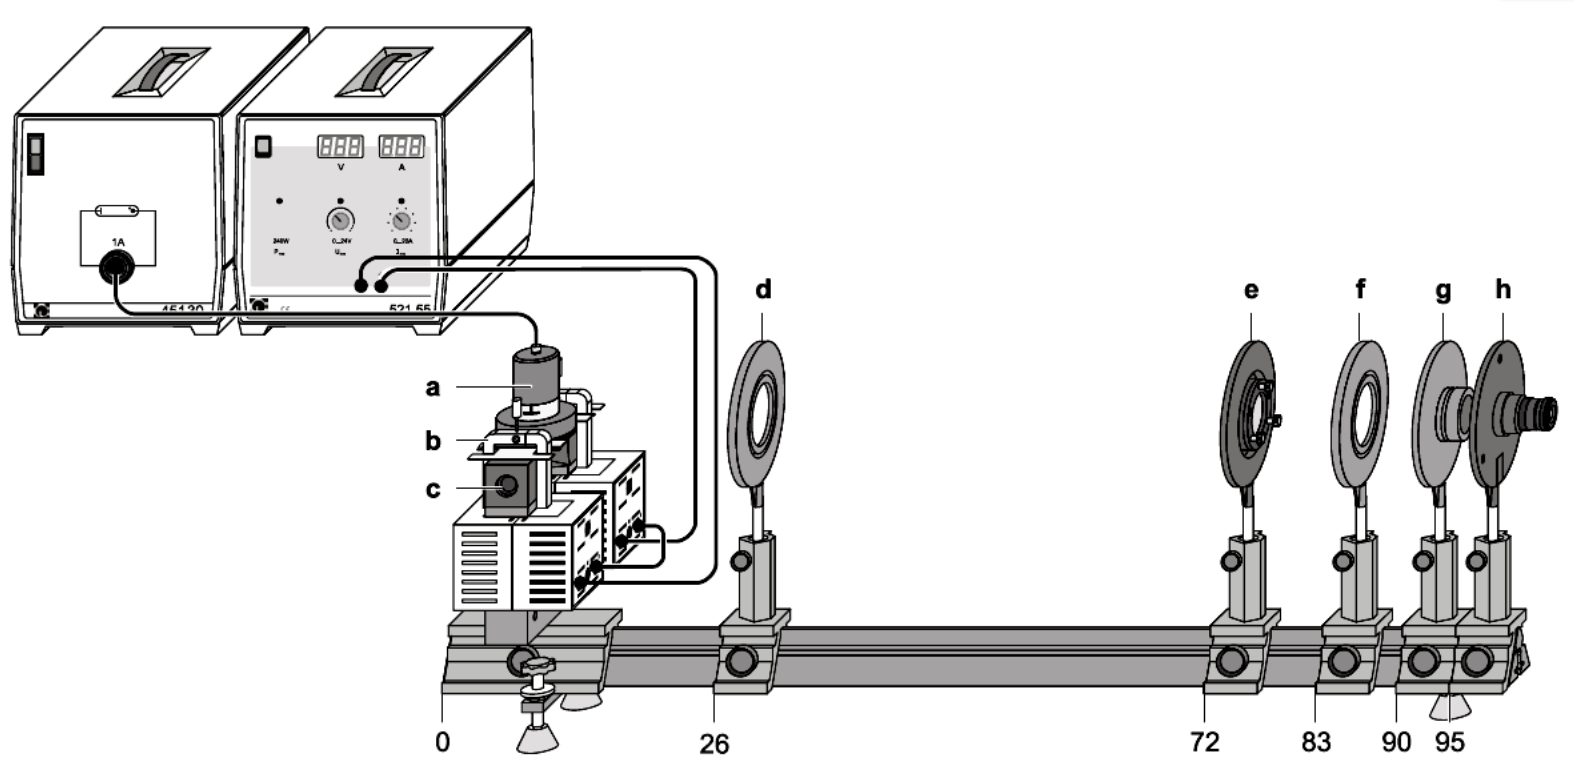
\includegraphics[width=\linewidth]{zeeman-aufbau}
  \caption{Versuchsaufbau Zeeman-Effekt \cite{Leybold}}
  \label{fig:zeeman-aufbau}
\end{figure}
% Der $^1D_2$-Zustand hat Aufspaltungen in $M_J = -2,\,\dots\,,2$ und $^1P_1$ in $M_J=-1,0,1$.
% Es kann also Übergänge mit $\Delta M_J = -1, 0, 1$ geben.
% In Abhängigkeit des $\Delta M$-Werts gibt es verschiedene
Folgende wichtige Bestandteile sind zu sehen \cite{Anleitung}:
\begin{enumerate}[label=\alph*.]
  \item Cadmium-Lampe
  \item Klammern
  \item Polschuhe
  \item Kondensorlinse
  \item Polarisationsfilter
  \item Fabry-Perot-Etalon
  \item Abbildungslinse
  \item Interferenzfilter ($\lambda=\SI{643.8}{\nm}$)
  \item Okular mit Strichskala
\end{enumerate}
Außerdem werden Stromquellen (oben links im Bild; links normal, rechts Hochstrom)
zur Versorgung der Cadmiumlampe und der Elektromagneten eingesetzt.

Das Fabry-Perot-Etalon in Kombination mit den Linsen erzeugt ein Interferenzmuster mit Ringen,
deren Position von der Wellenlänge des Lichts abhängt.
Der Interferenzfilter wird eingesetzt, um ausschließlich das Licht vom Übergang $^1D_2 \rightarrow\,^1P_1$ betrachten zu können.

Zur Justage des Aufbaus wird am Okular die Strichskala scharfgestellt und
die Abbildungslinse verschoben, bis das Interferenzmuster der Lampe durch das Etalon scharf zu sehen ist.
Das Etalon wird so gedreht, dass das Zentrum des Musters am Nullpunkt der Strichskala ist
und die Kondensorlinse verschoben, um eine gleichmäßige Ausleuchtung zu erhalten.

\subsection{Beobachtung des Zeeman-Effekts}
\subsubsection{transversale Konfiguration}
Zunächst wird in transversaler Konfiguration ohne eingesetzten Polarisationsfilter beobachtet,
d.h. die optische Achse steht senkrecht zum Magnetfeld, wie in Abb. \ref{fig:zeeman-aufbau} gezeigt.
Nach Abb. \ref{fig:zeeman-abstrahlung} sollte hier sowohl Strahlung vom $\Delta M_J=0$-Übergang ($\pi$-Übergang),
als auch den $\Delta M_J=\pm 1$-Übergängen ($\sigma^\pm$-Übergänge), zu sehen sein.
Hierbei ist die Strahlung der beiden verschiedenen $\sigma$-Übergänge gleich Polarisiert;
die Polarisation vom $\pi$-Übergang steht senkrecht dazu.

\begin{figure}[H]
  \centering
  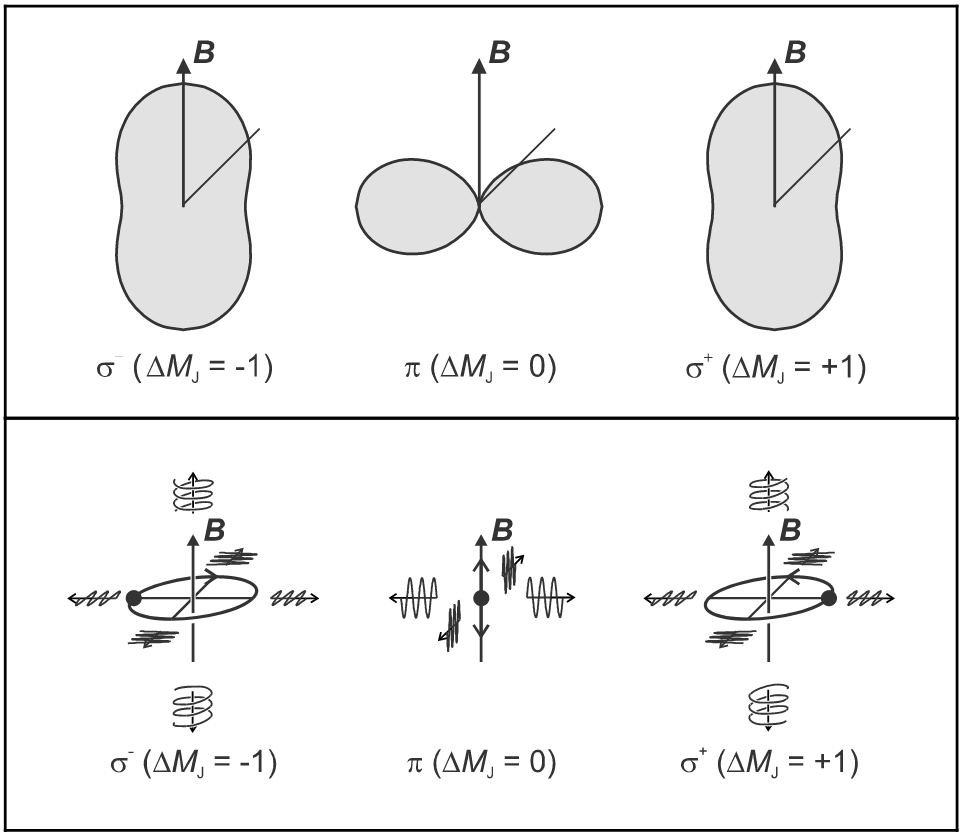
\includegraphics[width=.8\linewidth]{zeeman-abstrahlung}
  \caption{Polarisationsverteilung und Abstrahlungscharakteristik elektrischer Dipolübergänge \cite{Anleitung} \cite{Leybold}.}
  \label{fig:zeeman-abstrahlung}
\end{figure}

Das am Okular enstehende Bild ist in Abb. \ref{fig:zeeman-transveral-ohne-ohne} gezeigt.
\begin{figure}[H]
  \centering
  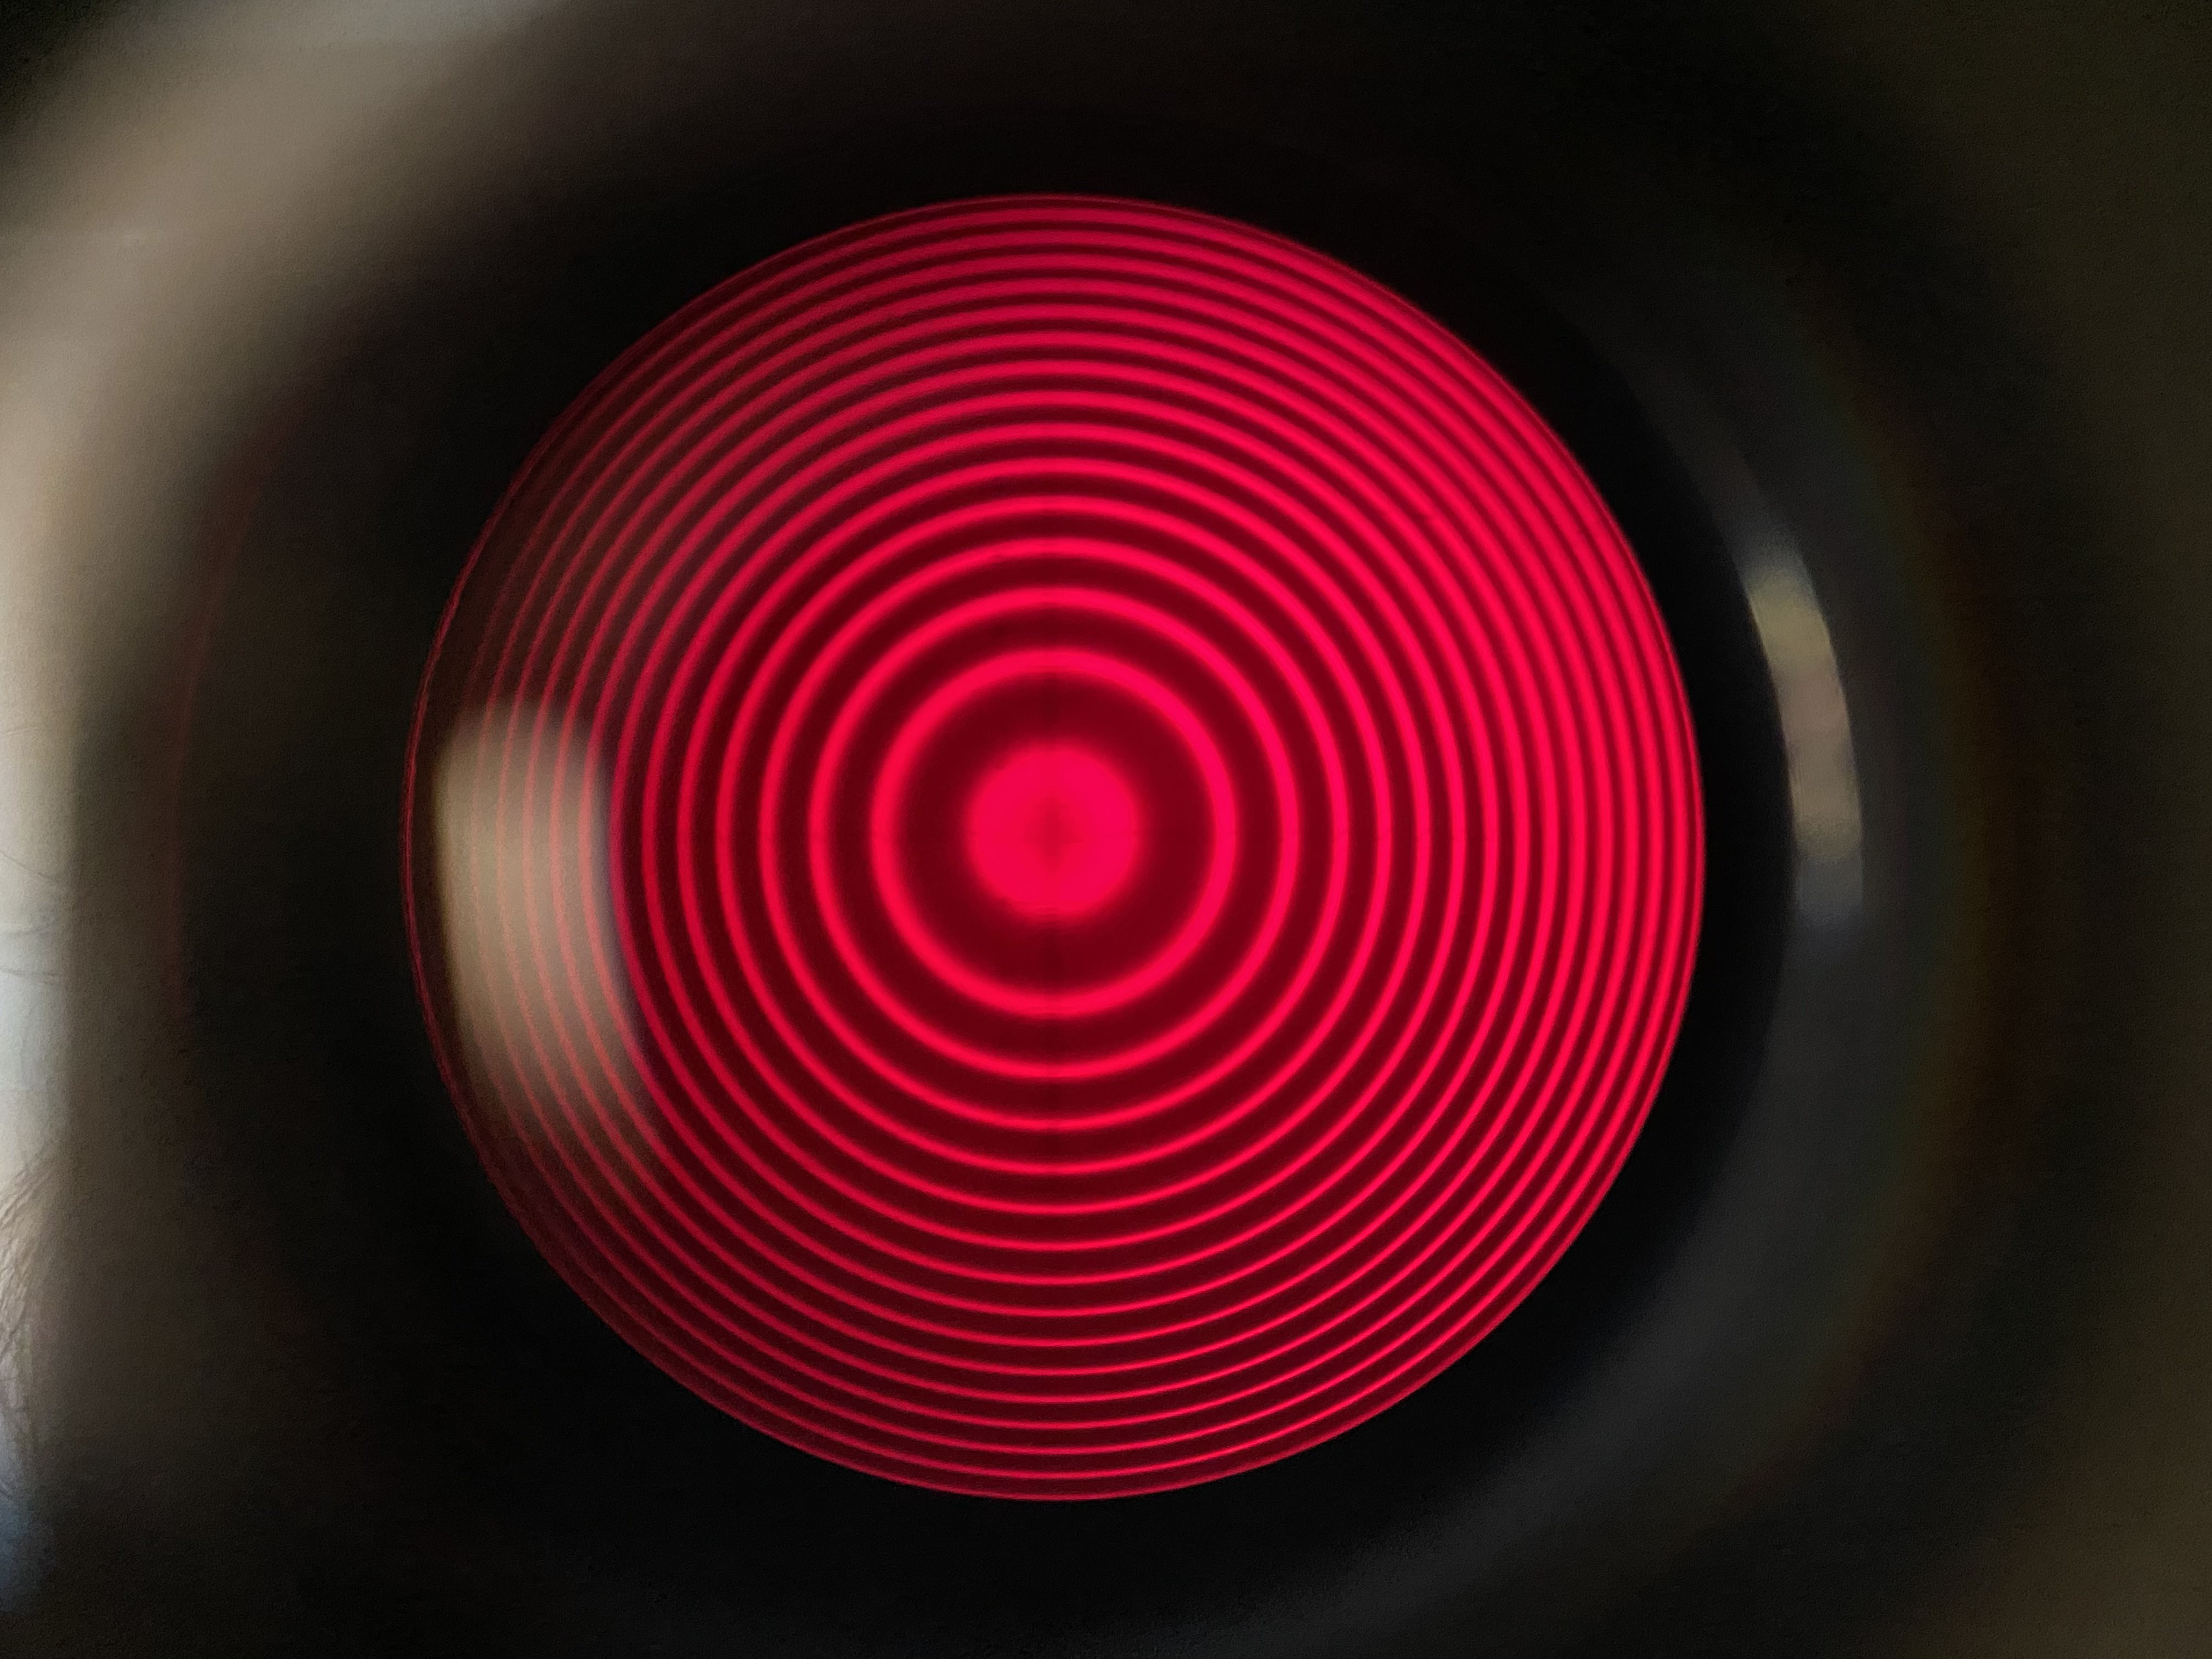
\includegraphics[width=.8\linewidth]{zeeman-transversal-ohne-ohne}
  \caption{Interferenzmuster bei transversaler Beobachtung ohne Magnetfeld, ohne Polarisationsfilter.}
  \label{fig:zeeman-transveral-ohne-ohne}
\end{figure}
Es sind die verschiedenen Interferenzringe zu erkennen, die hier alle von der gleichen Wellenlänge stammen.

Nun wird das Magnetfeld eingeschaltet und erhöht, bis man eine Aufspaltung der Ringe sieht, siehe Abb. \ref{fig:zeeman-transveral-mit-ohne}
\begin{figure}[H]
  \centering
  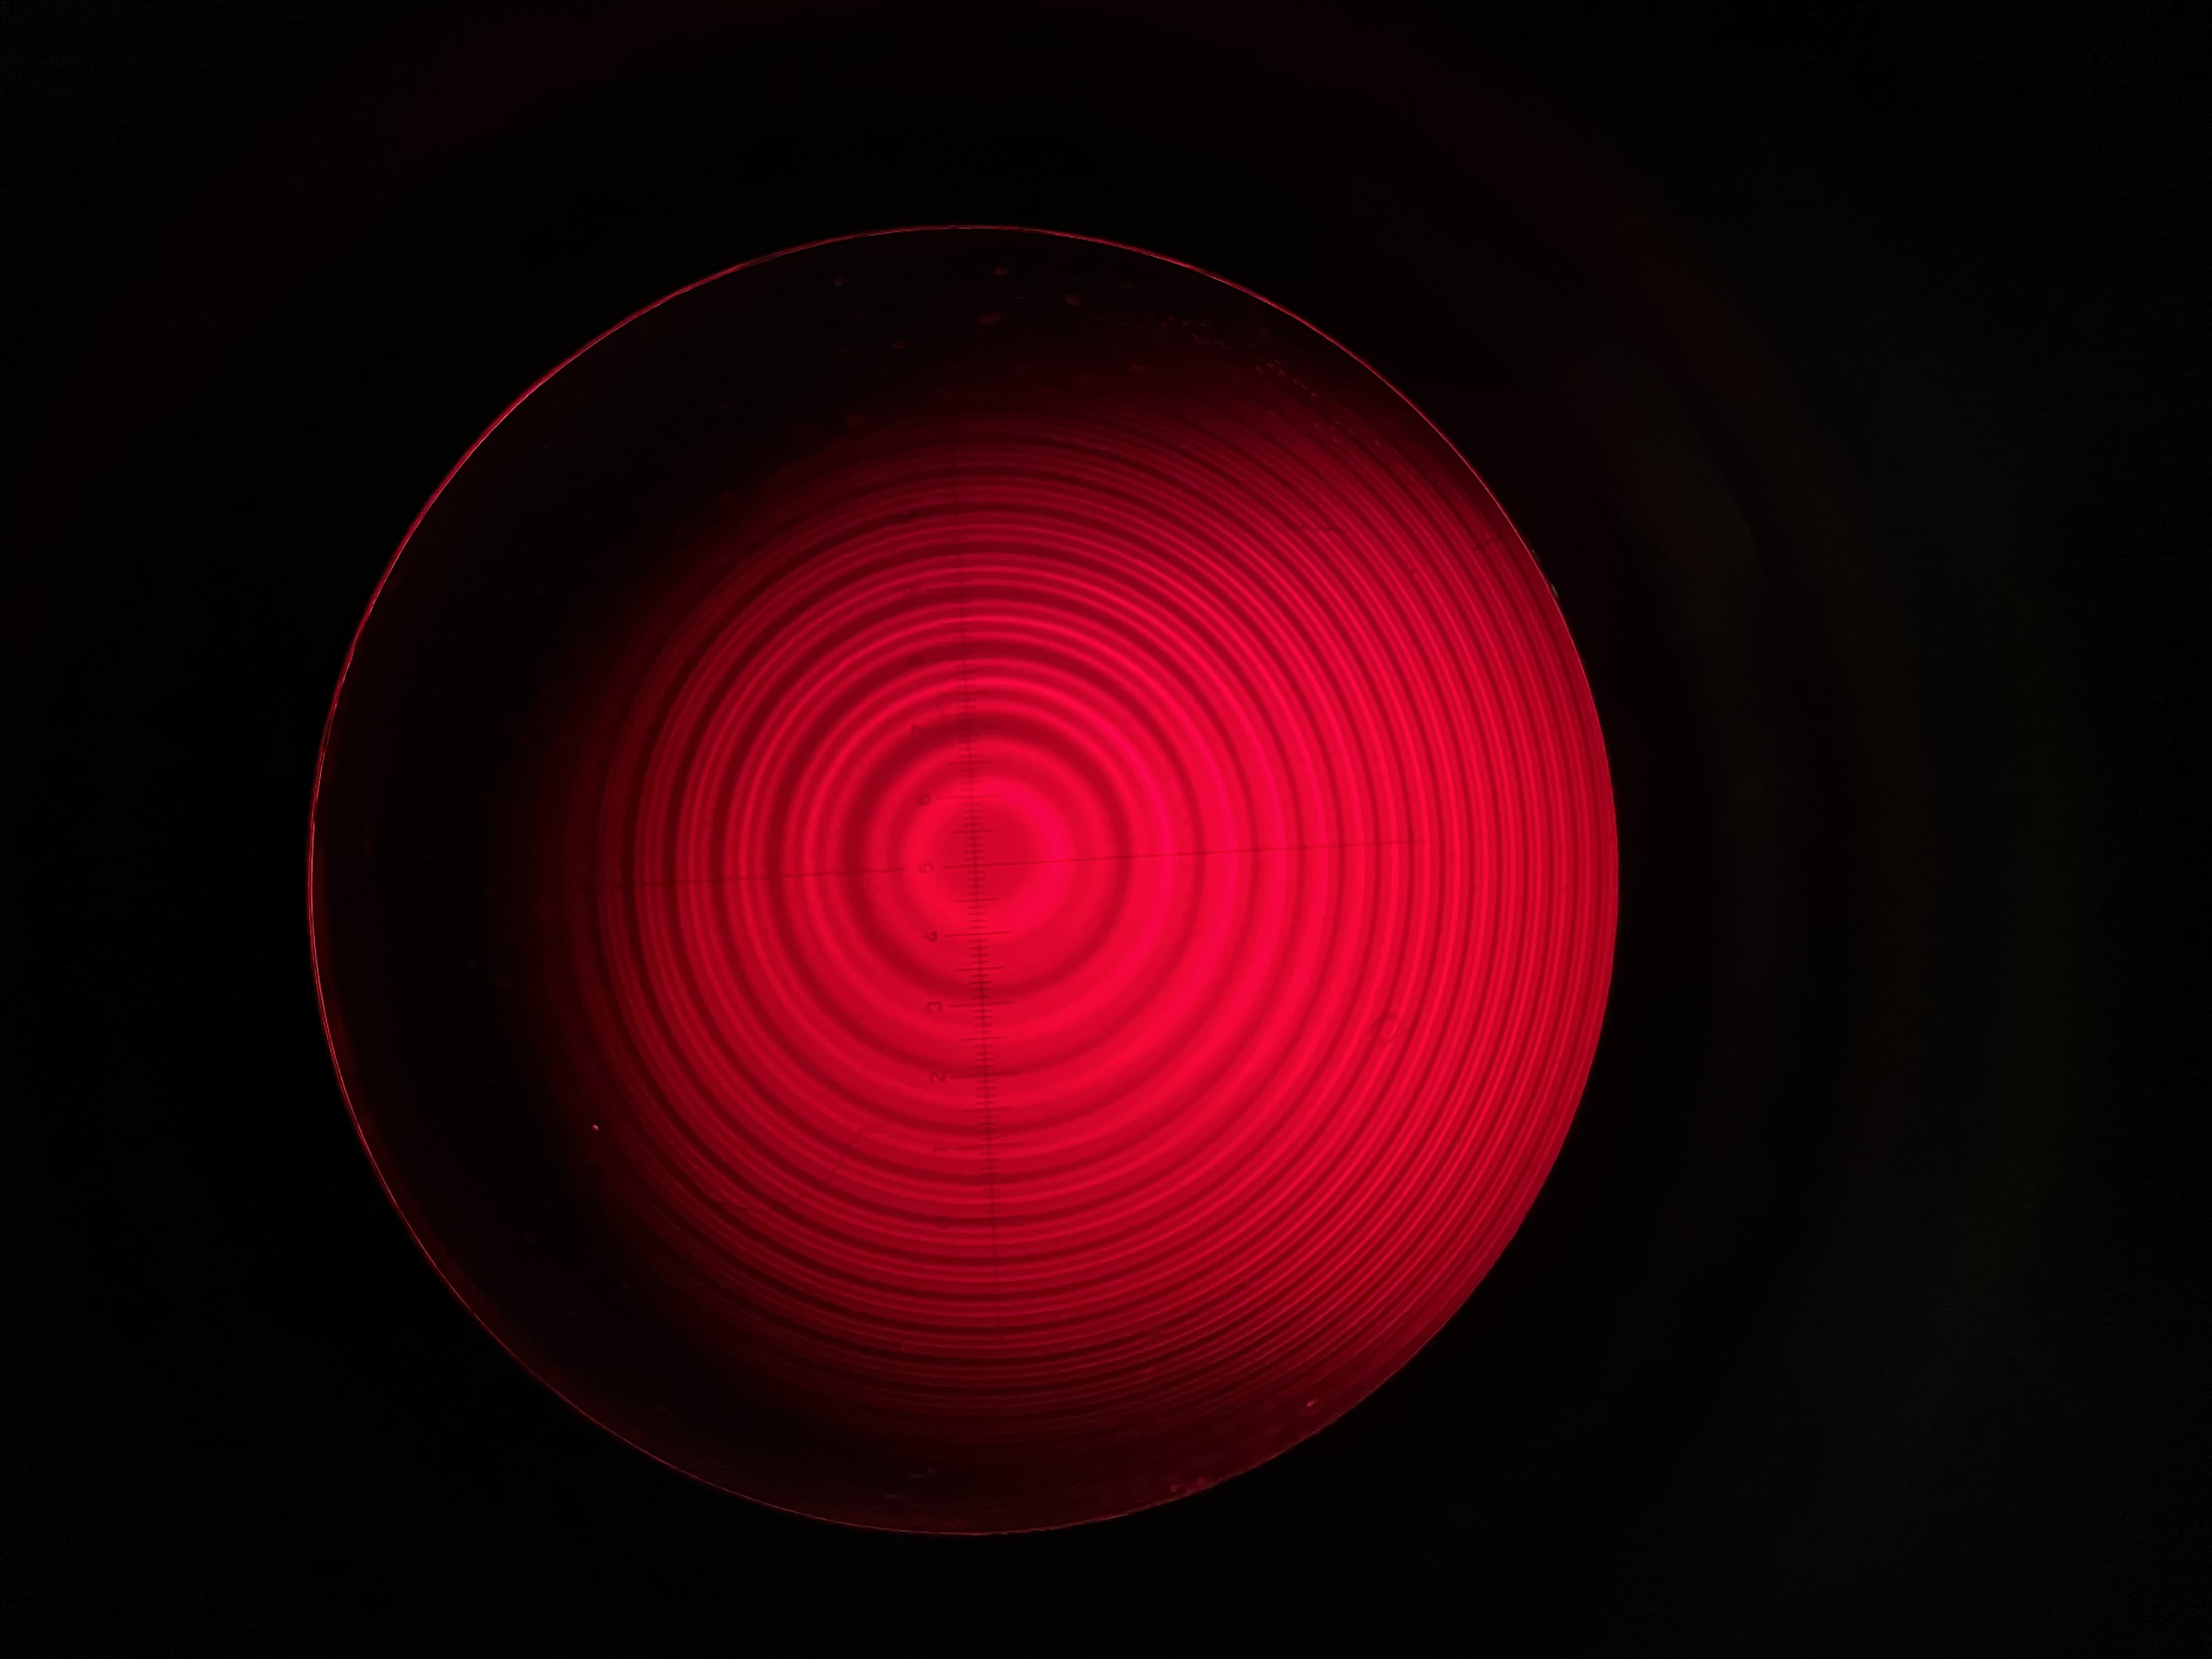
\includegraphics[width=.8\linewidth]{zeeman-transversal-mit-ohne}
  \caption{Interferenzmuster bei transversaler Beobachtung mit Magnetfeld, ohne Polarisationsfilter.}
  \label{fig:zeeman-transveral-mit-ohne}
\end{figure}
Durch den Zeeman-Effekt gibt es eine Energieaufspaltung $\Delta E \propto B_zM_J$ der Niveaus.
Dadurch sind die $\pi$-Übergänge unbeeinflusst, während die $\sigma^+$- bzw. $\sigma^-$-Übergänge
eine etwas geringere bzw. höhere Wellenlänge produzieren. Was zuvor ein Ring war, spaltet sich daher in drei Ringe auf.

Die verschiedenen Komponenten können durch Einsatz des Polarisationsfilters herausgefiltert werden (Abb. \ref{fig:zeeman-transveral-mit-90}, \ref{fig:zeeman-transveral-mit-0}).
\begin{figure}[H]
  \centering
  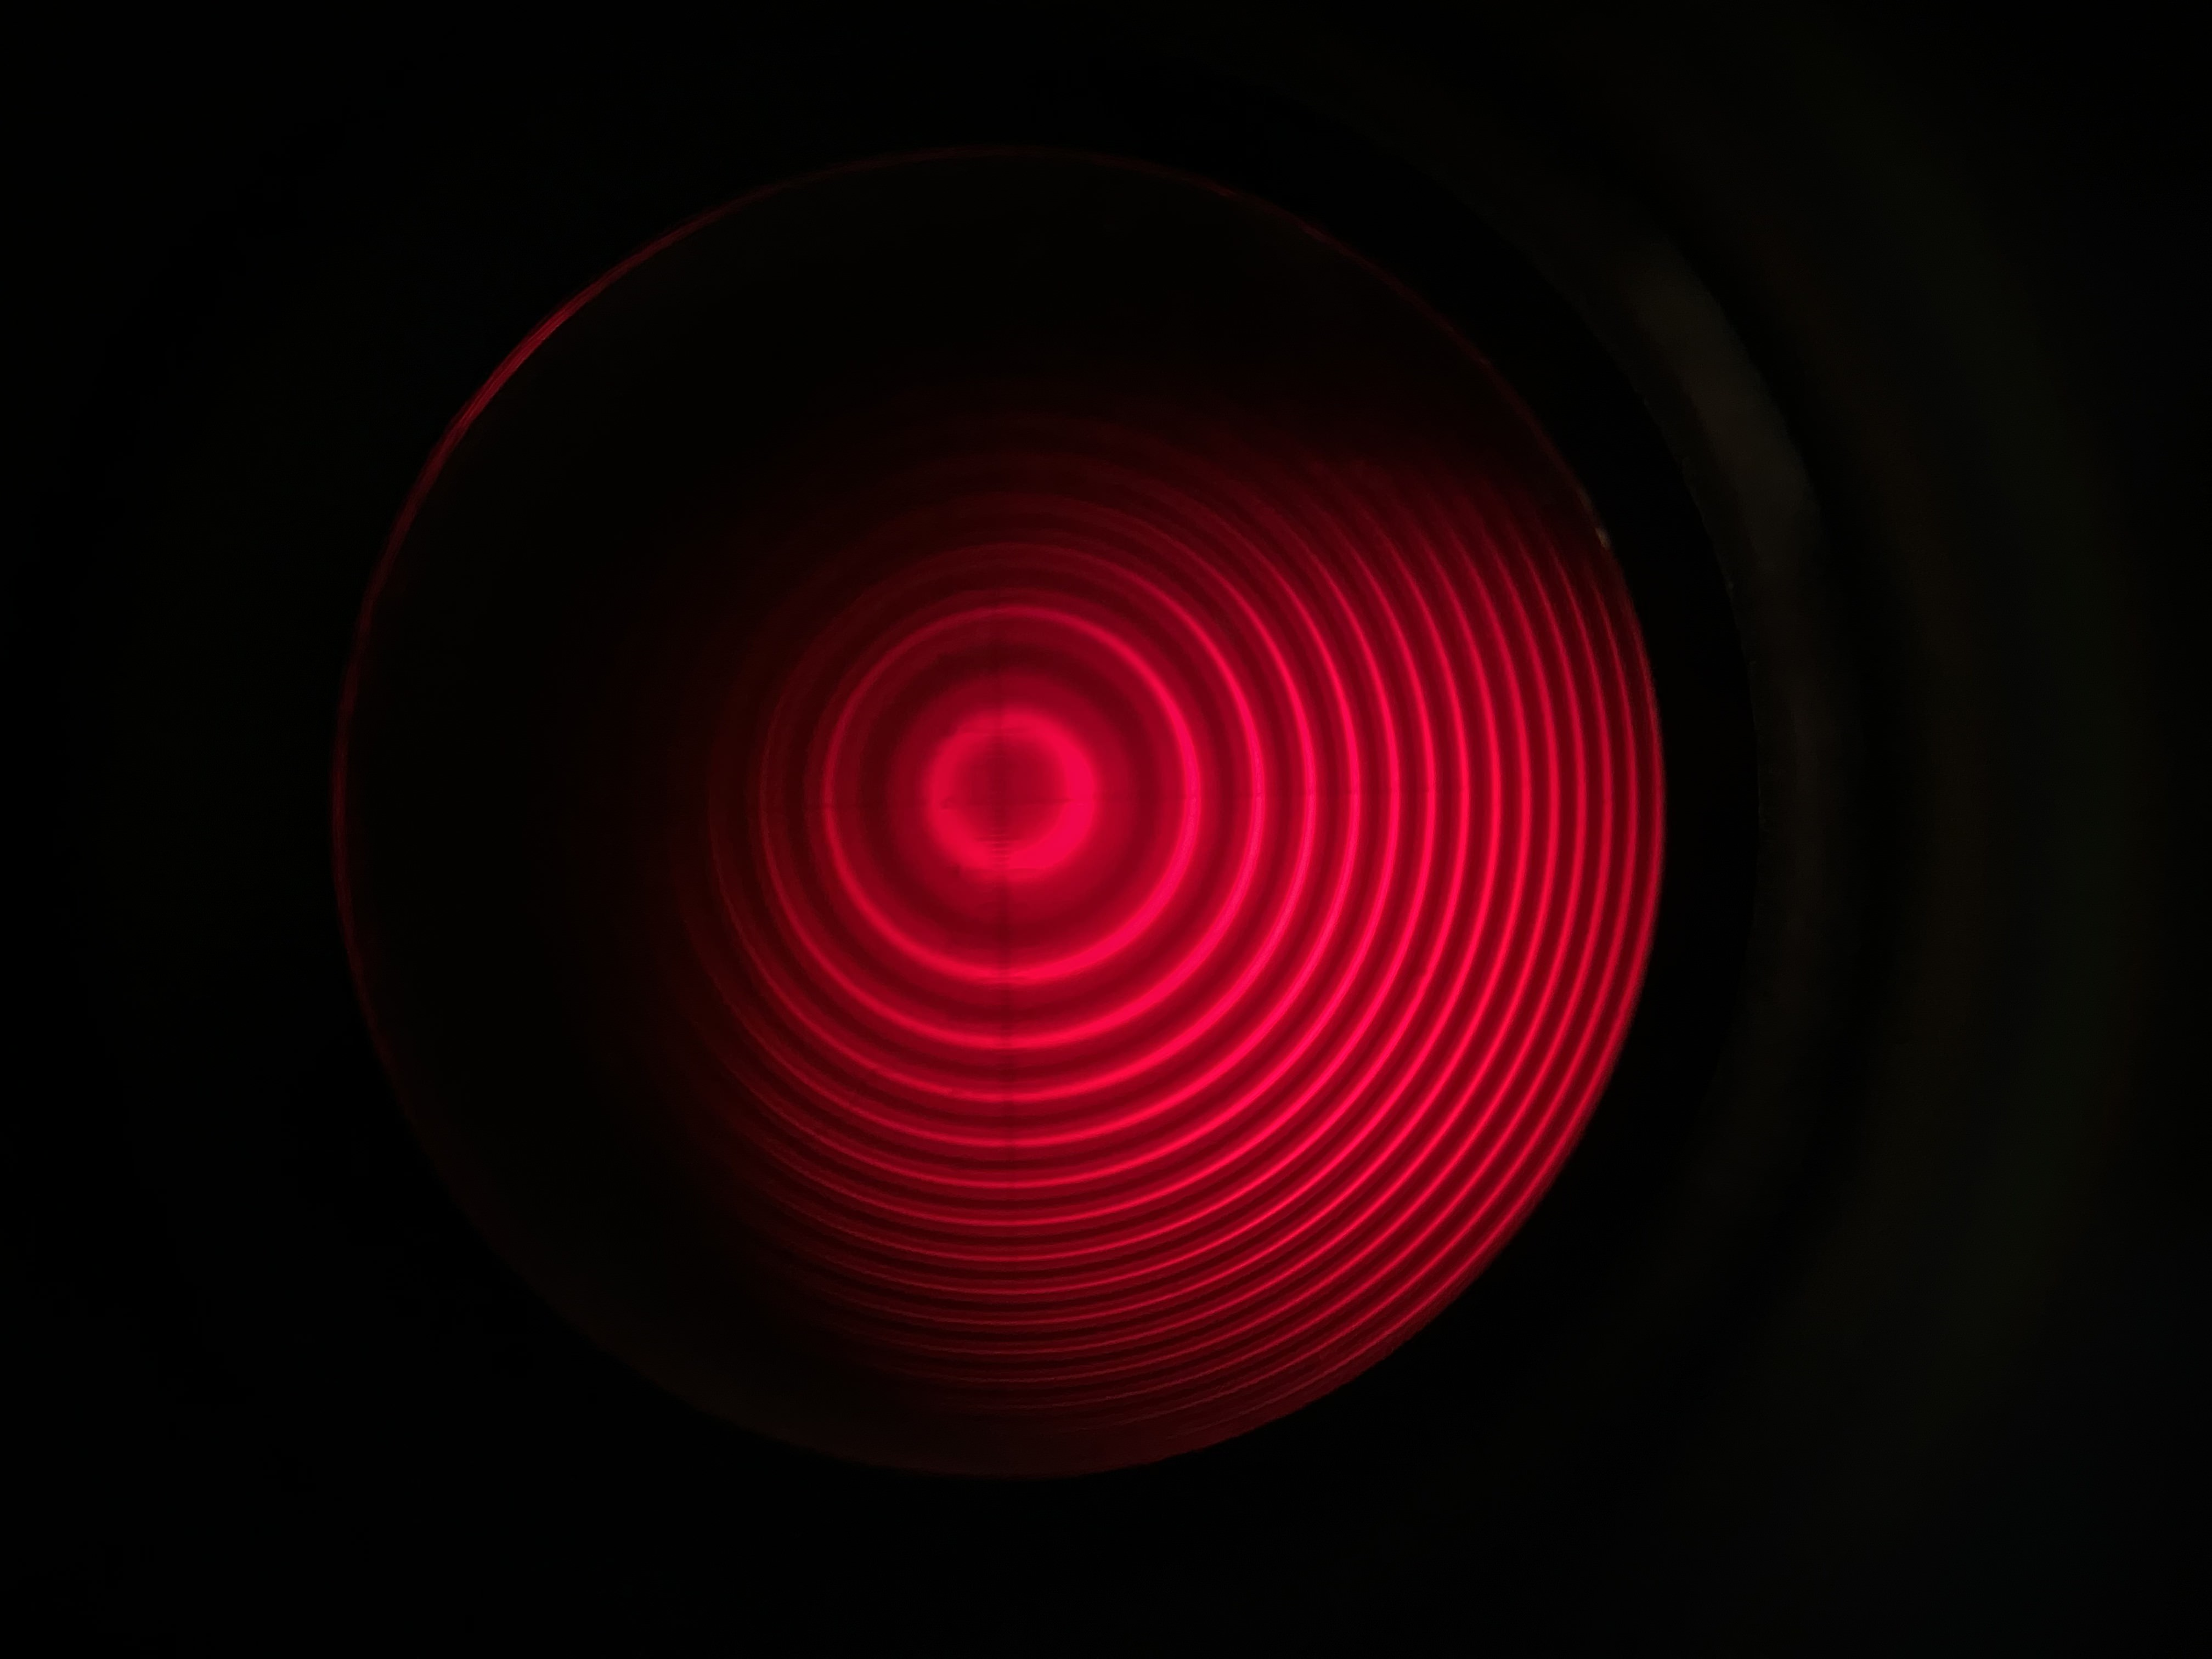
\includegraphics[width=.8\linewidth]{zeeman-transversal-mit-90}
  \caption{Interferenzmuster bei transversaler Beobachtung mit Magnetfeld, mit Polarisationsfilter auf \ang{90}.}
  \label{fig:zeeman-transveral-mit-90}
\end{figure}
\begin{figure}[H]
  \centering
  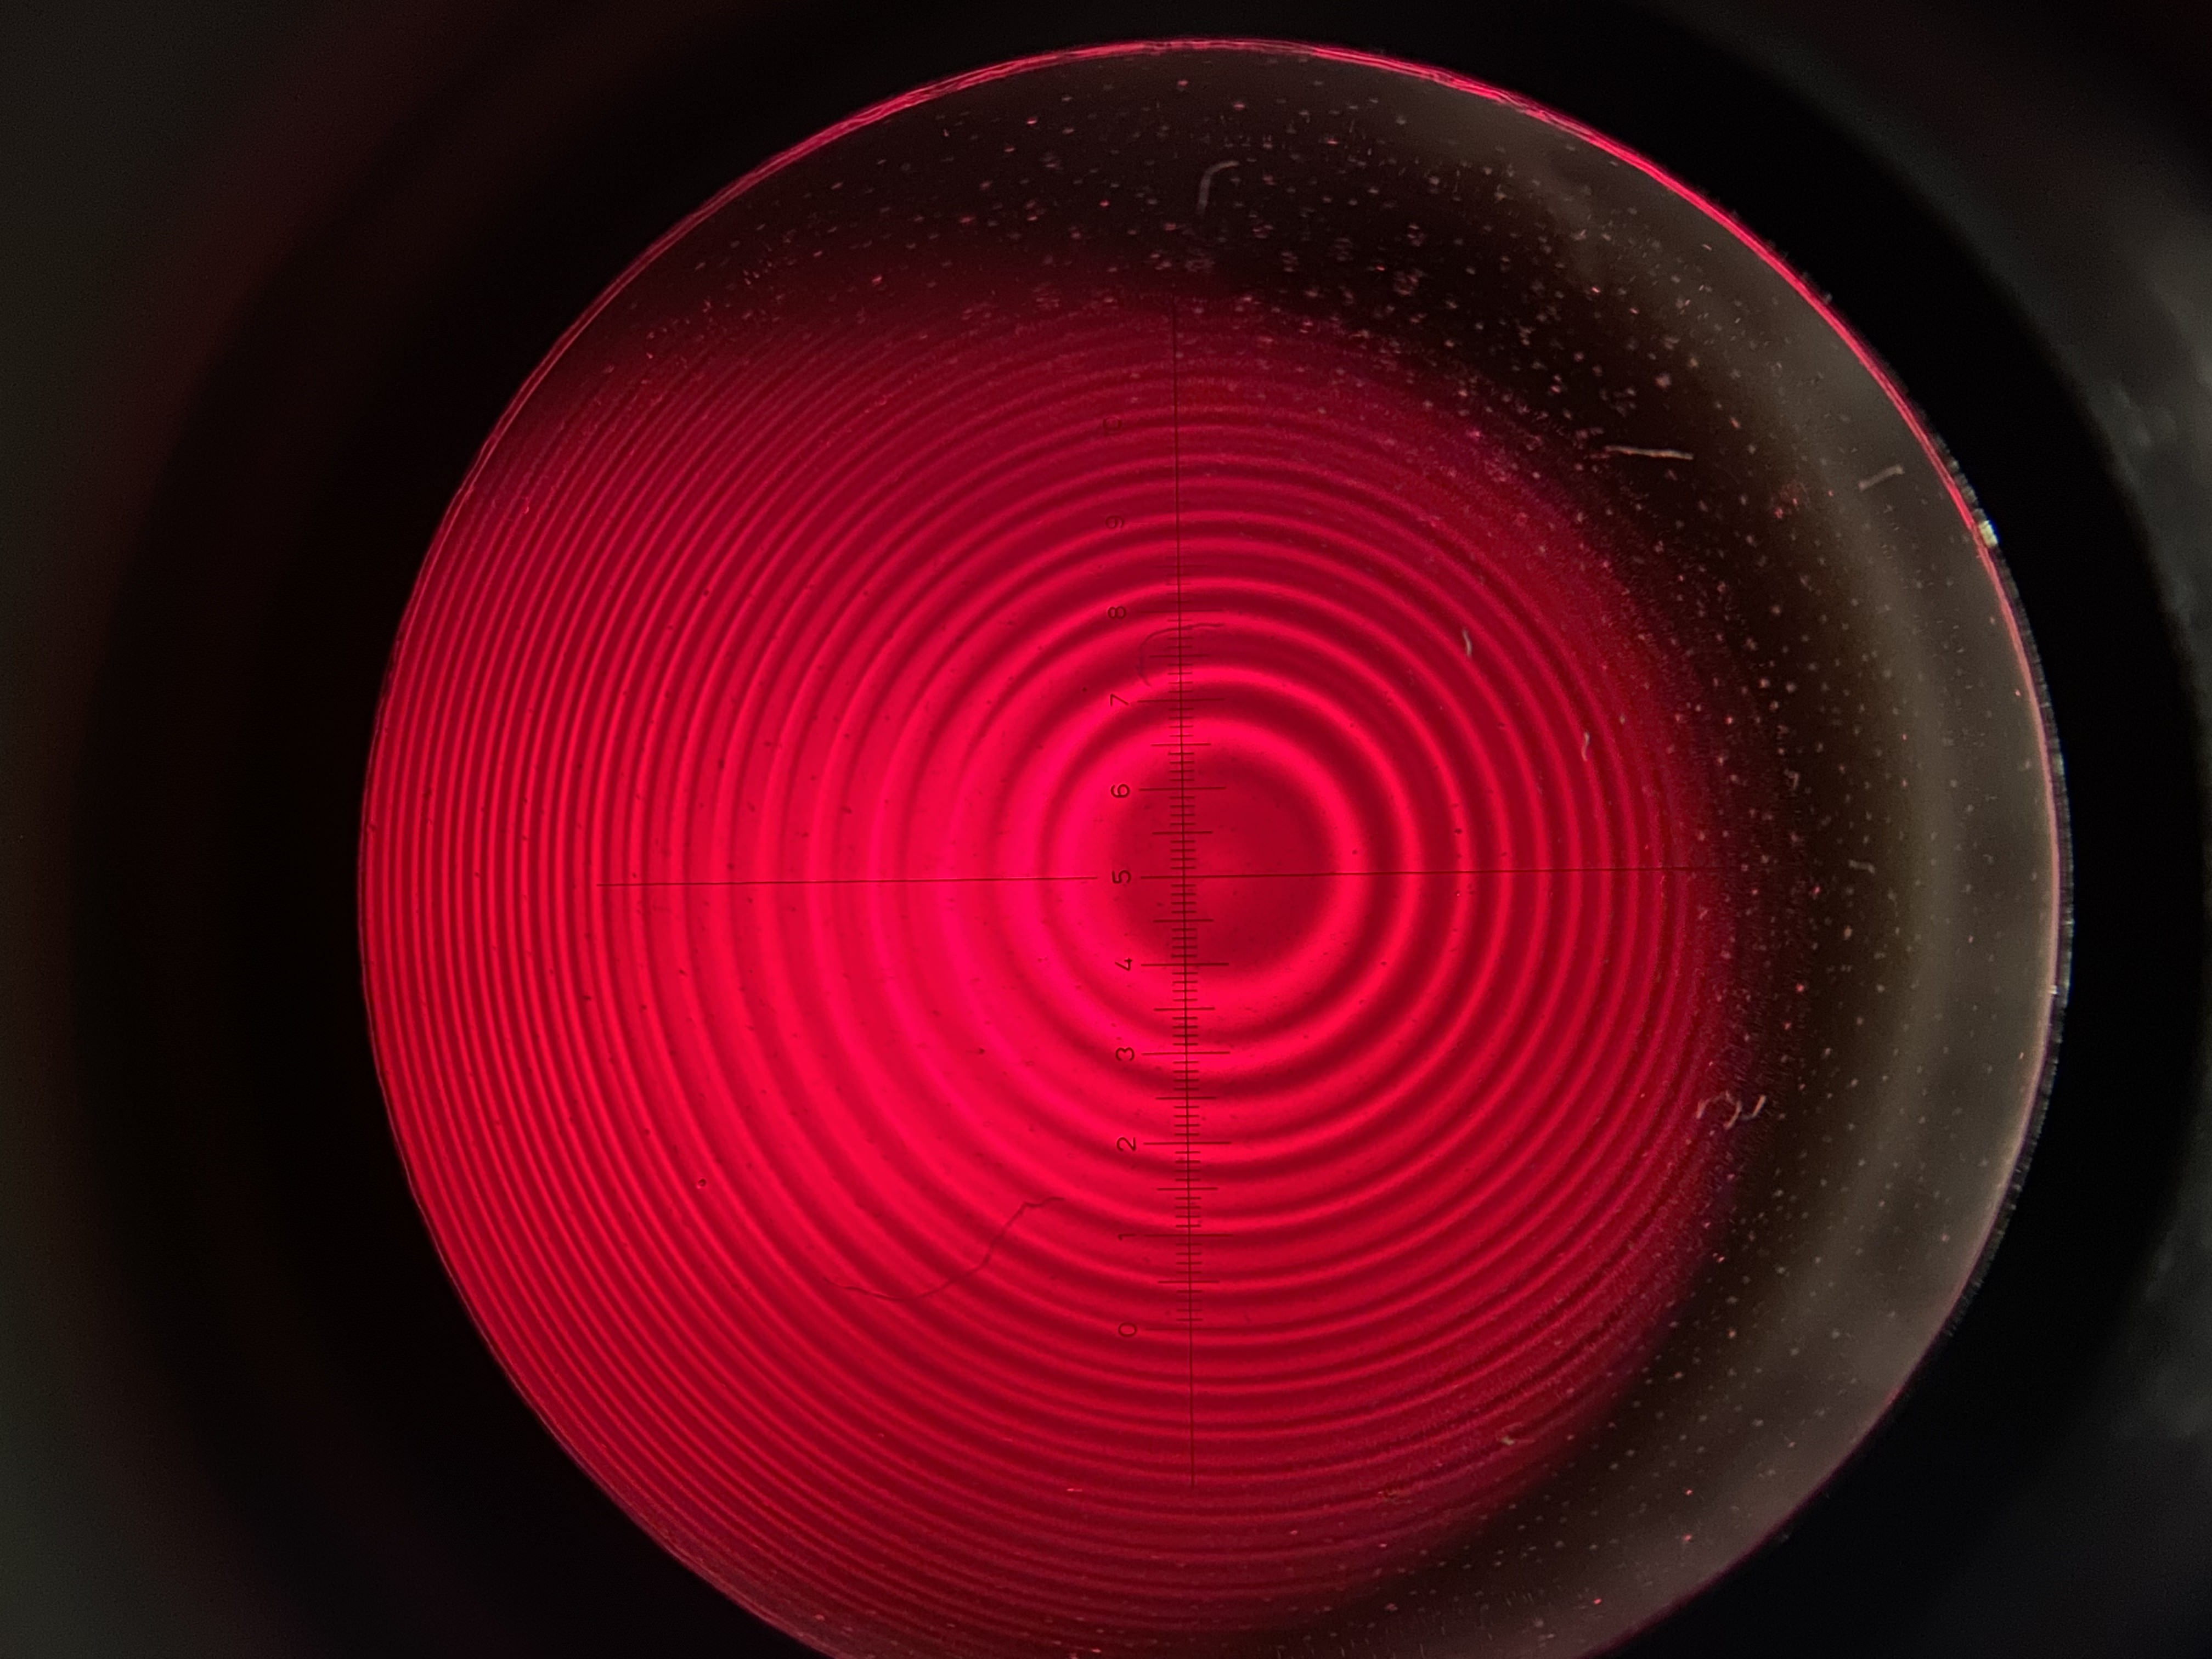
\includegraphics[width=.8\linewidth]{zeeman-transversal-mit-0}
  \caption{Interferenzmuster bei transversaler Beobachtung mit Magnetfeld, mit Polarisationsfilter auf \ang{0}.}
  \label{fig:zeeman-transveral-mit-0}
\end{figure}
Wenn der Filter auf \ang{90} steht, sind wieder nur einzelne Ringe zu sehen, die dem $\pi$-Übergang entsprechen,
welche Licht mit Polarisation parallel zum Magnetfeld produziert.
Steht der Filter auf \ang{0}, gibt es jeweils zwei Ringe, die $\sigma^+$ bzw. $\sigma^-$ entsprechen.

\subsection{Auflösungsvermögen und Finesse}

Nach dem Praktikumskript ist Dicke von Fabry-Perot-Etalon 
$d = 4 \, \text{mm}$, die Mittelwellenlänge $\lambda = 643.8 \, \text{nm}$ und 
für Reflexiongrad $R=0.85$.
Damit lässt sich das theoretische Auflösungsvermögen und die Finesse $F$ 
bestimmen, es gilt dann:
\[
F_{\text{theo}} = \frac{\pi R}{1 - R^2}= 9.63
\]
\[
  A_{\text{theo}} = \frac{F \cdot 2nd}{\lambda} = 1.742 \cdot 10^5
\]

Wie im Protokoll beschrieben wird, wird der Strom so eingestellt, sodass die Aufspaltung
Spektralinien sich unterscheiden können.
\[
I_{\text{long}} = (1.2 \pm 0.1) \, \text{A}, \quad I_{\text{trans}} = (2.4 \pm 0.2) \, \text{A}
\]
Noch dazu ist der Wert des Magnetfeldes nach der Kalibrierung das Folgende: 
\[
B_{\text{long}} = ( 83.45 \pm 6.66) \, \text{mT}, \quad B_{\text{trans}} = (173.1 \pm 13.9) \, \text{mT}
\]

Zuletzt mit $A=\frac{hc}{\mu_B \lambda B}$ (und mit $\cdot \frac{1}{2}$ bei longitudinale 
Konfiguration) sind die jeweiligen Auflösungsvermögen und Finesse die folgende:
\[
A_{\text{trans}} = (1.88 \pm 0.14) \cdot 10^5, \quad A_{\text{long}} = (1.19 \pm 0.13) \cdot 10^5
\]
\[
  F_{\text{trans}} = 10.61 \pm 0.14 \, \text{N}, F_{\text{long}} = 6.72 \pm 0.13 \, \text{N}
\]
Unsere Werte sind ähnlich, was es zu erwarten war, denn Unsere Werte für 
$B_i$ das doppelte sind. Jedoch sind unsere beiden Werte zu niedrig gefallen und 
könnte an der Messgenauigkeit liegen. 

\subsection{Dopplerverbreiterung}


\subsubsection{longitudinale Konfiguration}
Die Magneten mitsamt der Cadmiumlampe werden um \ang{90} gedreht,
um die Beobachtungen in longitudinaler Konfiguration (Magnetfeld parallel zur optischen Achse bzw. der Beobachtungsrichtung)
zu wiederholen.

Ohne Magnetfeld ergibt sich das Muster in Abb. \ref{fig:zeeman-longitudinal-ohne-ohne}, was mit der entsprechenden Beobachtung
bei transversaler Konfiguration übereinstimmt.
\begin{figure}[H]
  \centering
  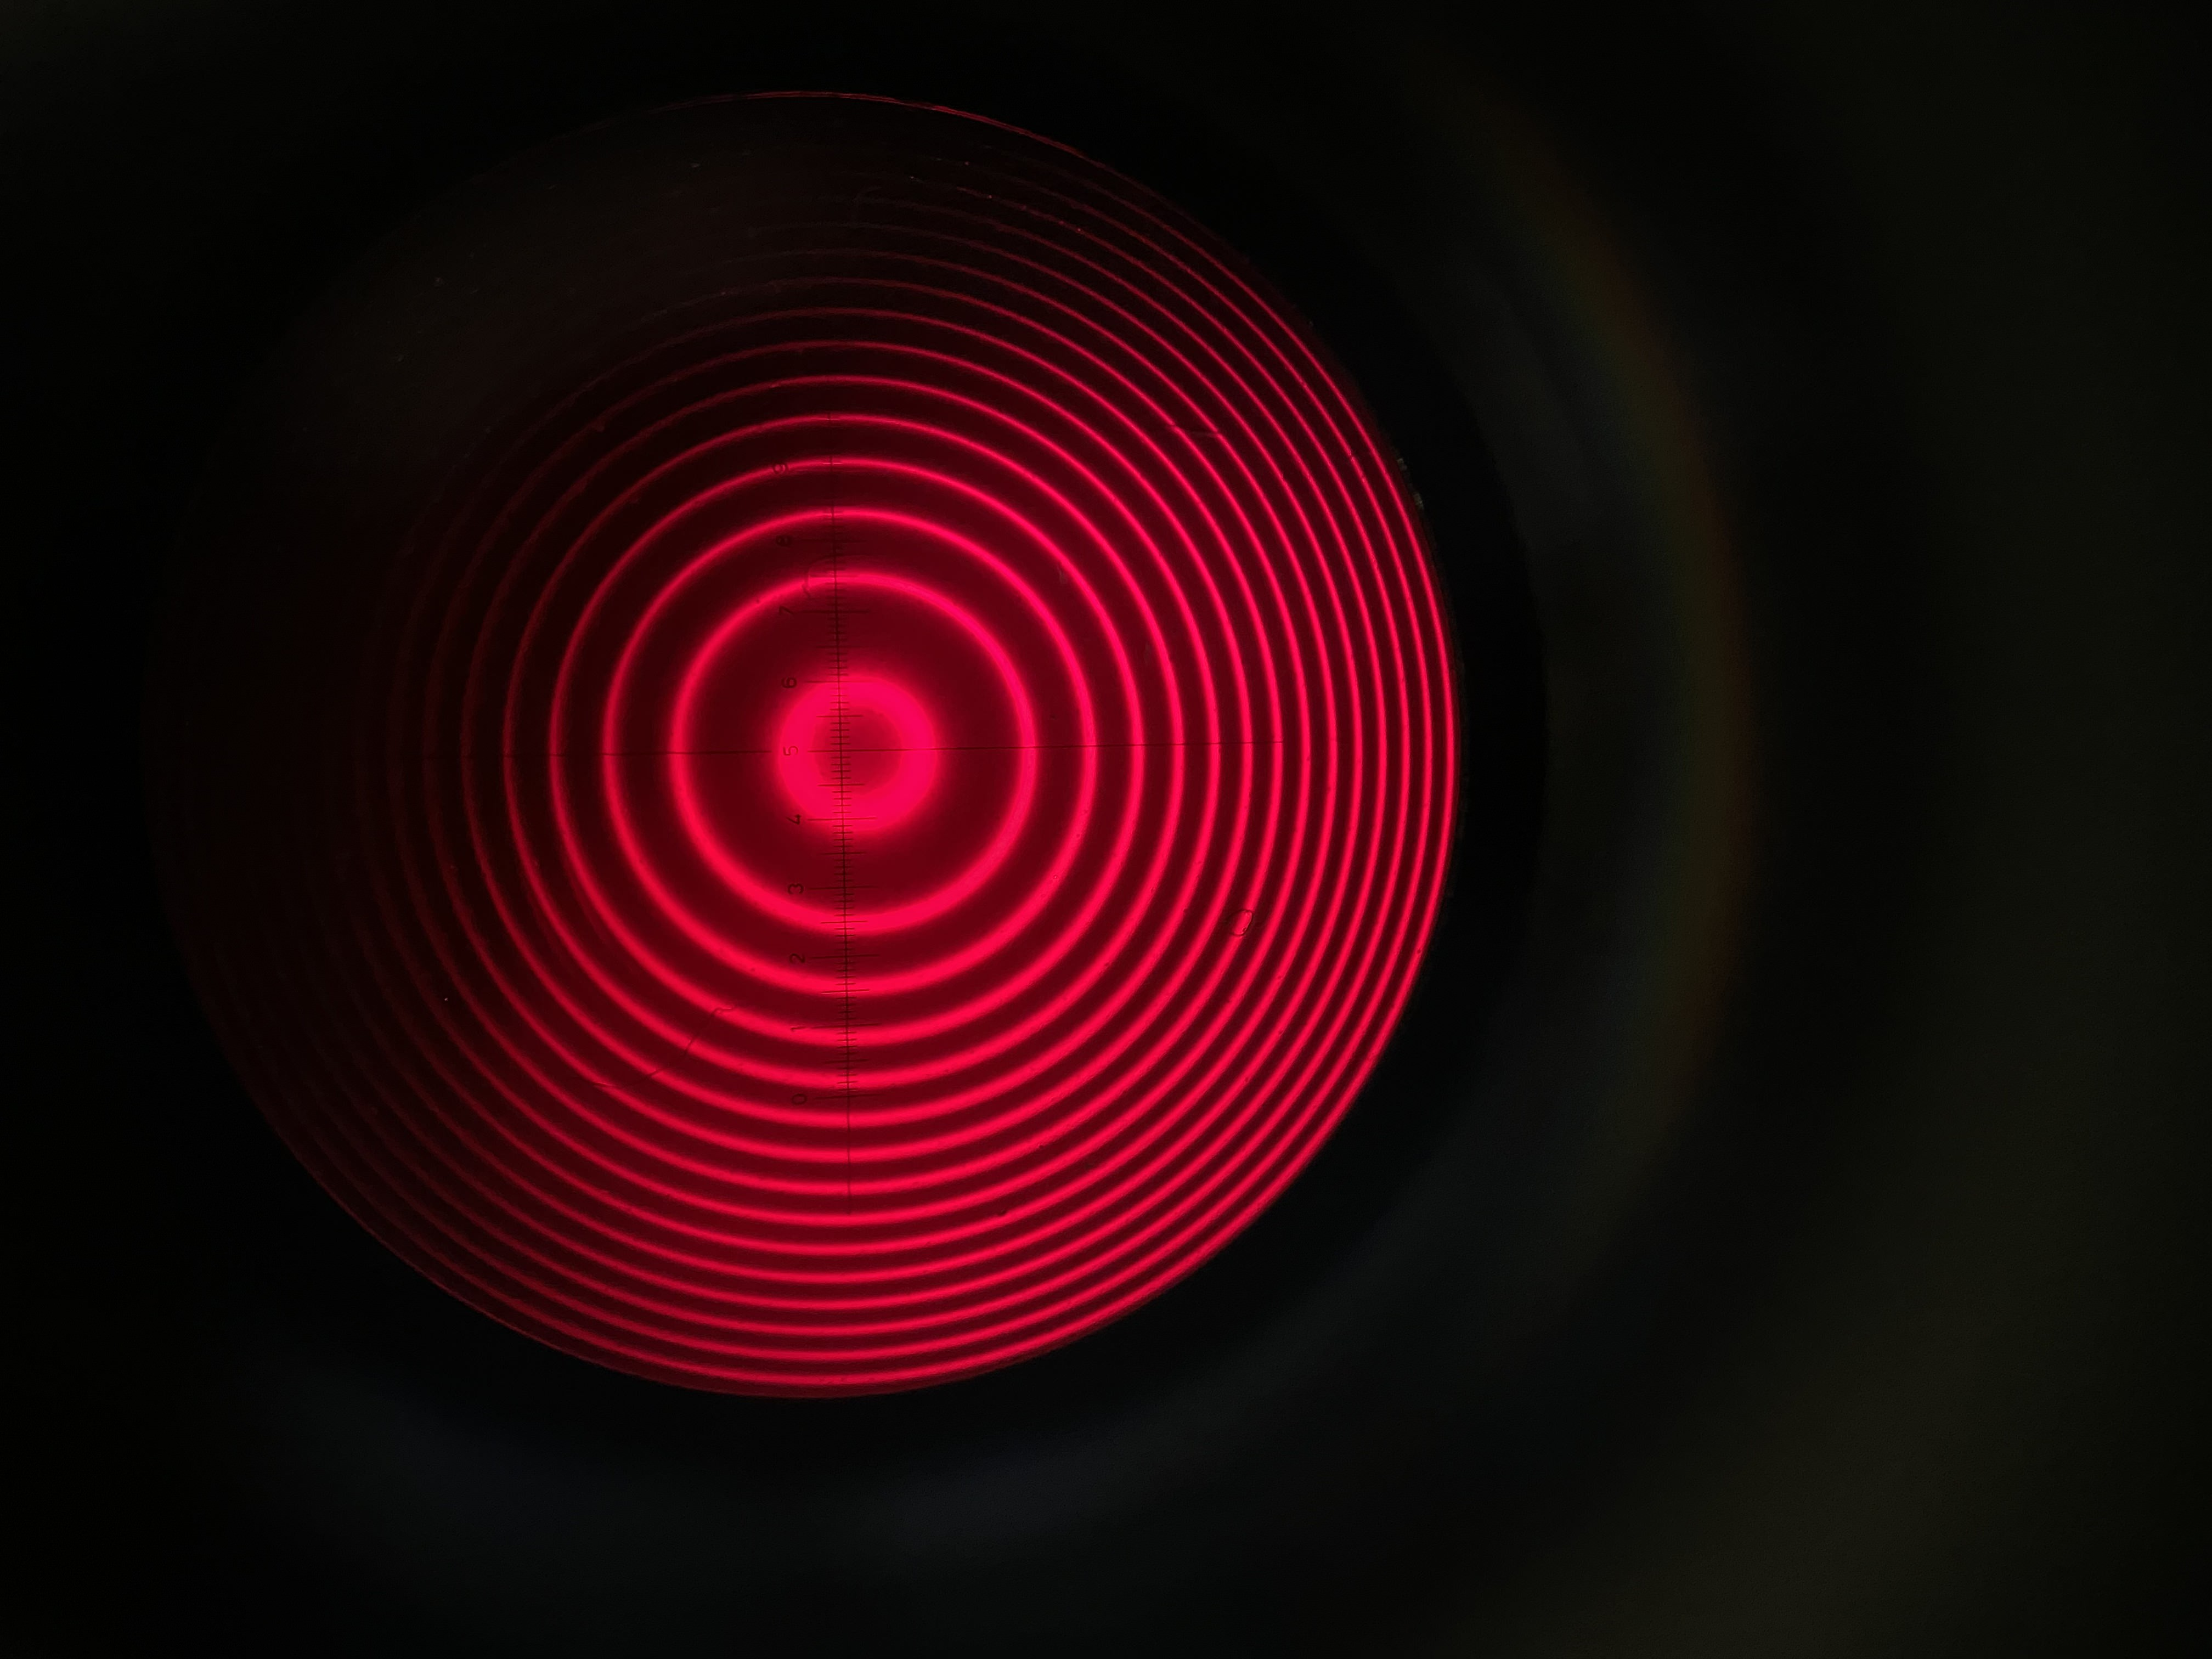
\includegraphics[width=.8\linewidth]{zeeman-longitudinal-ohne-ohne}
  \caption{Interferenzmuster bei longitudinaler Beobachtung ohne Magnetfeld, ohne Polarisationsfilter.}
  \label{fig:zeeman-longitudinal-ohne-ohne}
\end{figure}

Wird das Magnetfeld angeschaltet (Abb. \ref{fig:zeeman-longitudinal-mit-ohne}), ist eine Aufspaltung in jeweils zwei Ringe zu beobachten.
Diese entsprechen den beiden $\sigma$-Übergängen, während der $\pi$-Übergang aufgrund seiner Abstrahlungscharakteristik
in longitudinaler Konfiguration nicht zu sehen ist.
\begin{figure}[H]
  \centering
  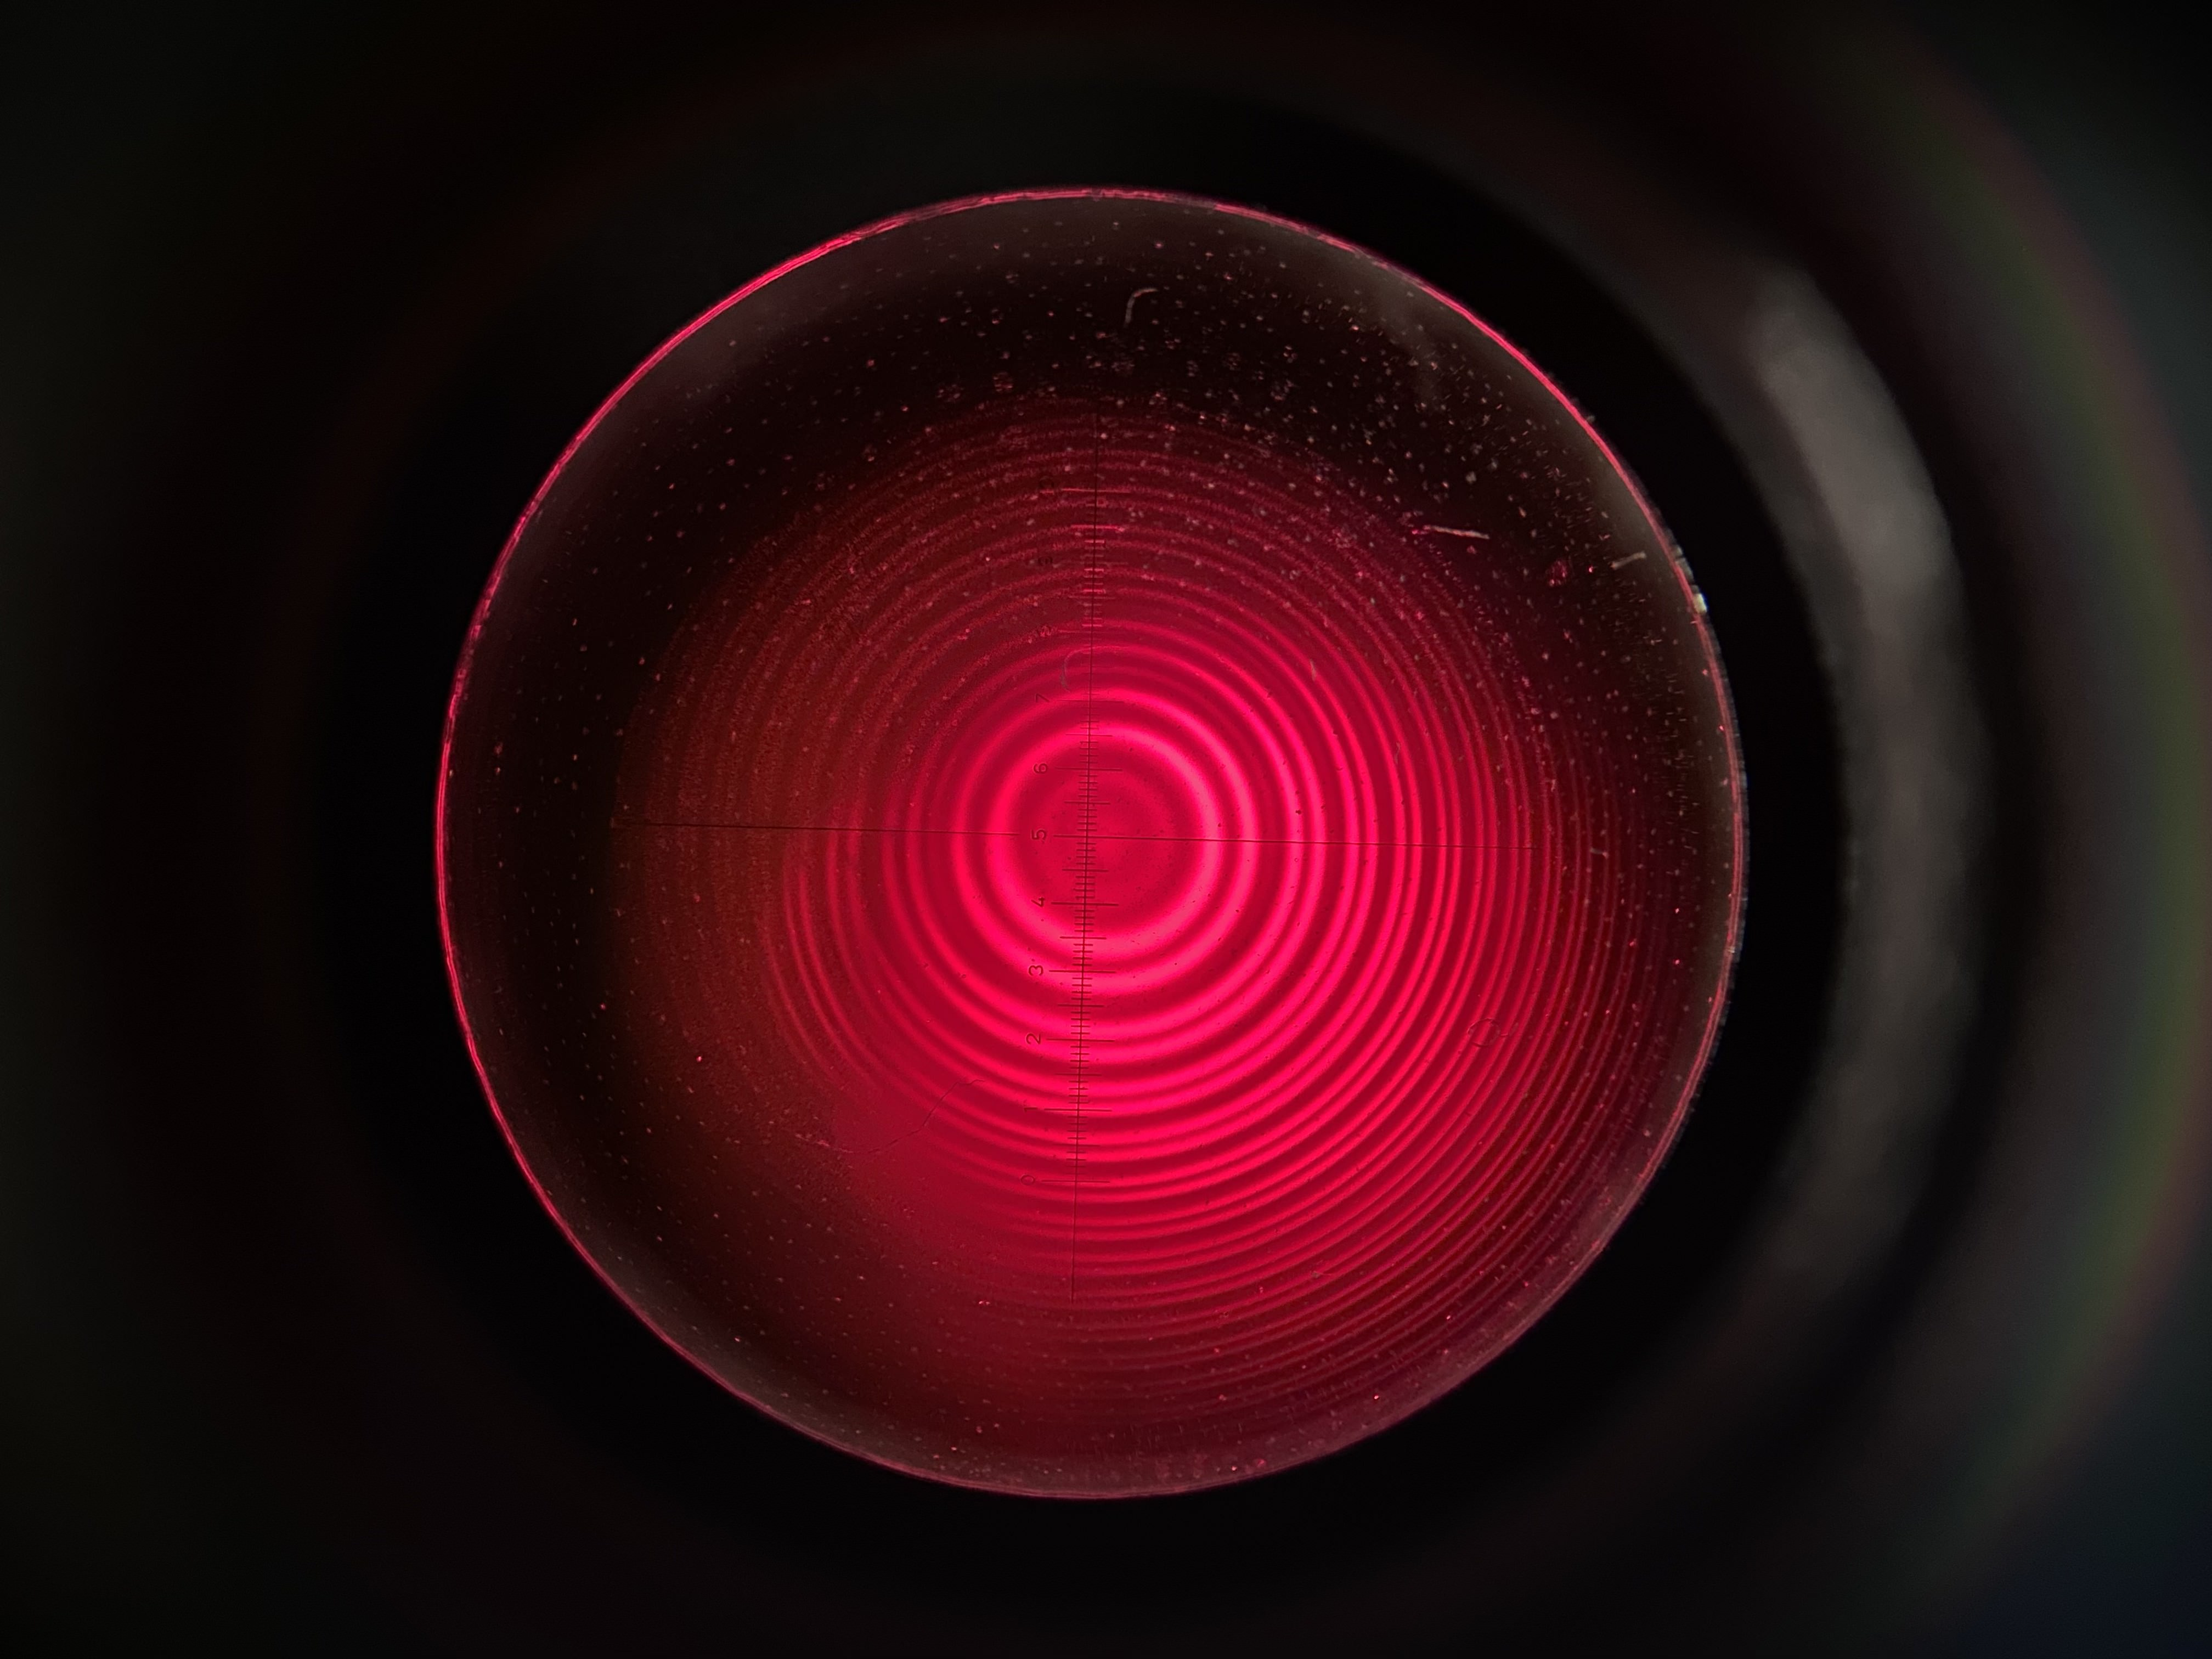
\includegraphics[width=.8\linewidth]{zeeman-longitudinal-mit-ohne}
  \caption{Interferenzmuster bei longitudinaler Beobachtung mit Magnetfeld, ohne Polarisationsfilter.}
  \label{fig:zeeman-longitudinal-mit-ohne}
\end{figure}

Als nächstes wird zusätzlich eine $\lambda / 4$-Platte in \ang{0}-Stellung in den Strahlengang vor dem
Polarisationsfilter eingesetzt. Diese dient dazu, das rechts- bzw. linkspolarisierte Licht der $\sigma$-Übergänge
(siehe Abb. \ref{fig:zeeman-abstrahlung}) zu verschiedenen linearen Polarisationsrichtungen umzuwandeln,
welche dann mit dem Polarisationsfilter ausgewählt werden können.

Mit dem Polarisationsfilter auf \ang{-45} ist nur noch jeweils ein Ring stark zu sehen (Abb. \ref{fig:zeeman-longitudinal-mit--45})
\begin{figure}[H]
  \centering
  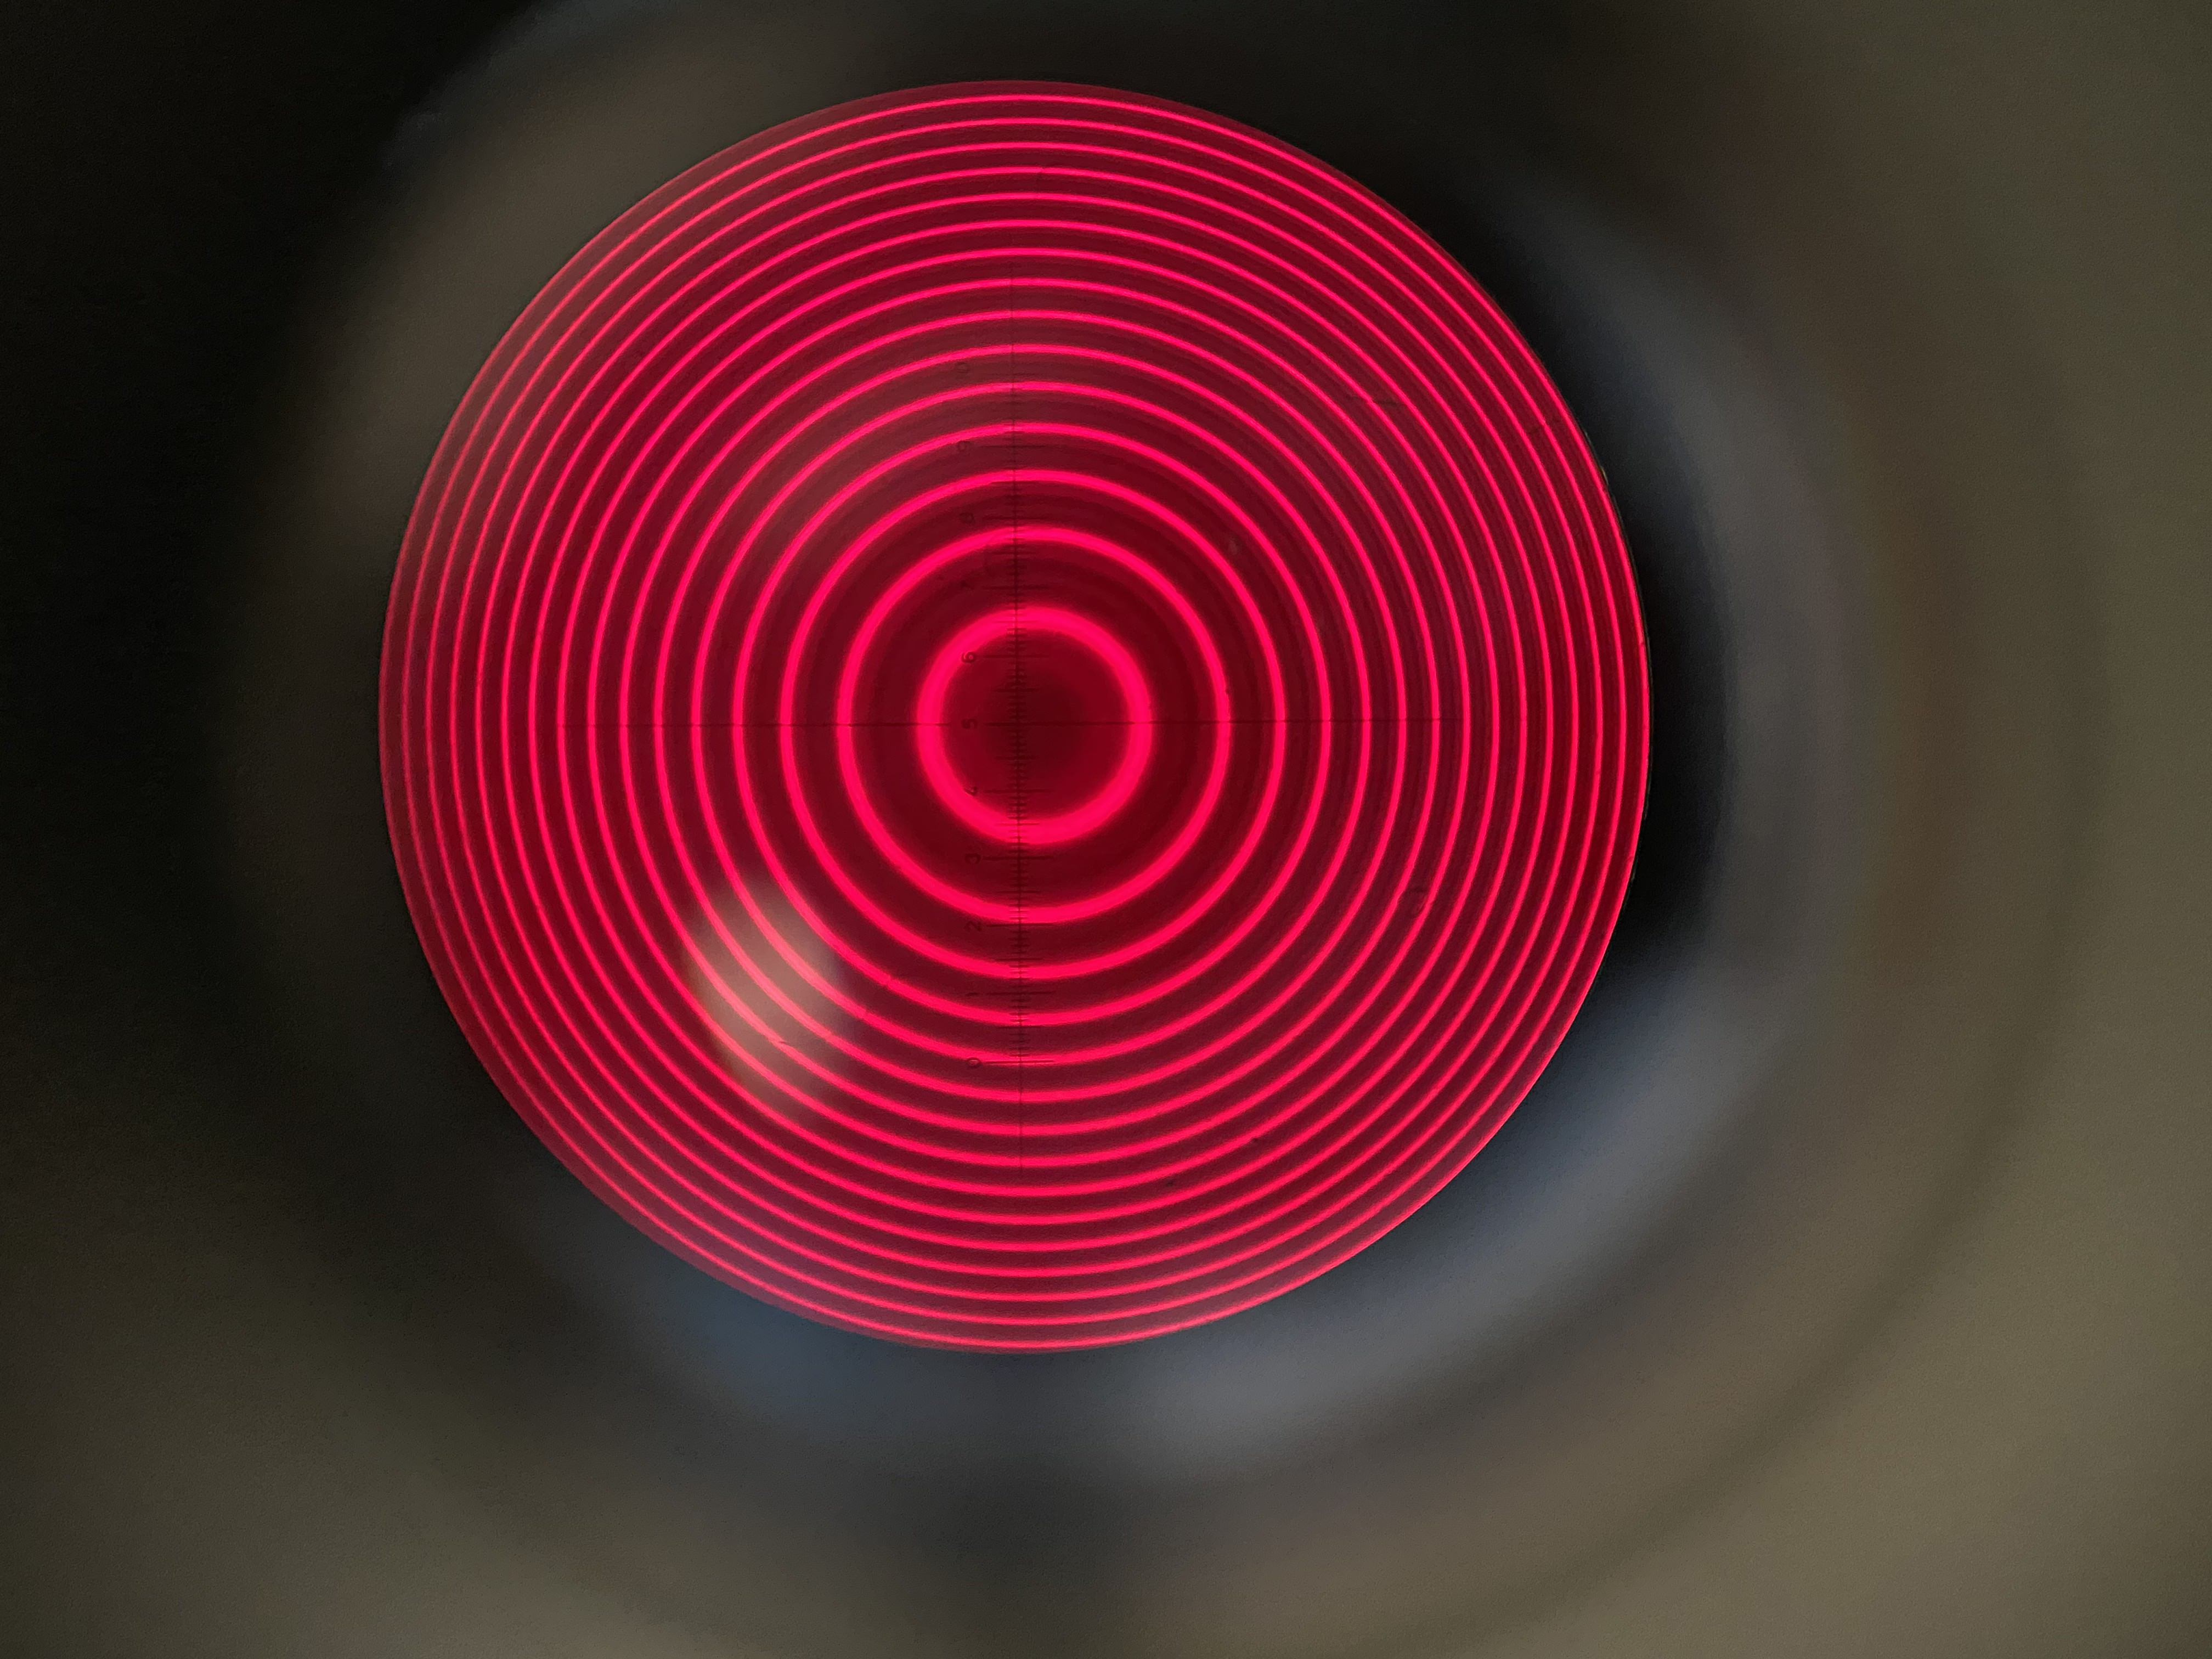
\includegraphics[width=.8\linewidth]{zeeman-longitudinal-mit--45}
  \caption{Interferenzmuster bei longitudinaler Beobachtung mit Magnetfeld, mit Polarisationsfilter.}
  \label{fig:zeeman-longitudinal-mit--45}
\end{figure}

Mit dem Polarisationsfilter in \ang{45}-Stellung ist nur der jeweils andere Ring stark zu sehen (Abb. \ref{fig:zeeman-longitudinal-mit-45}).
\begin{figure}[H]
  \centering
  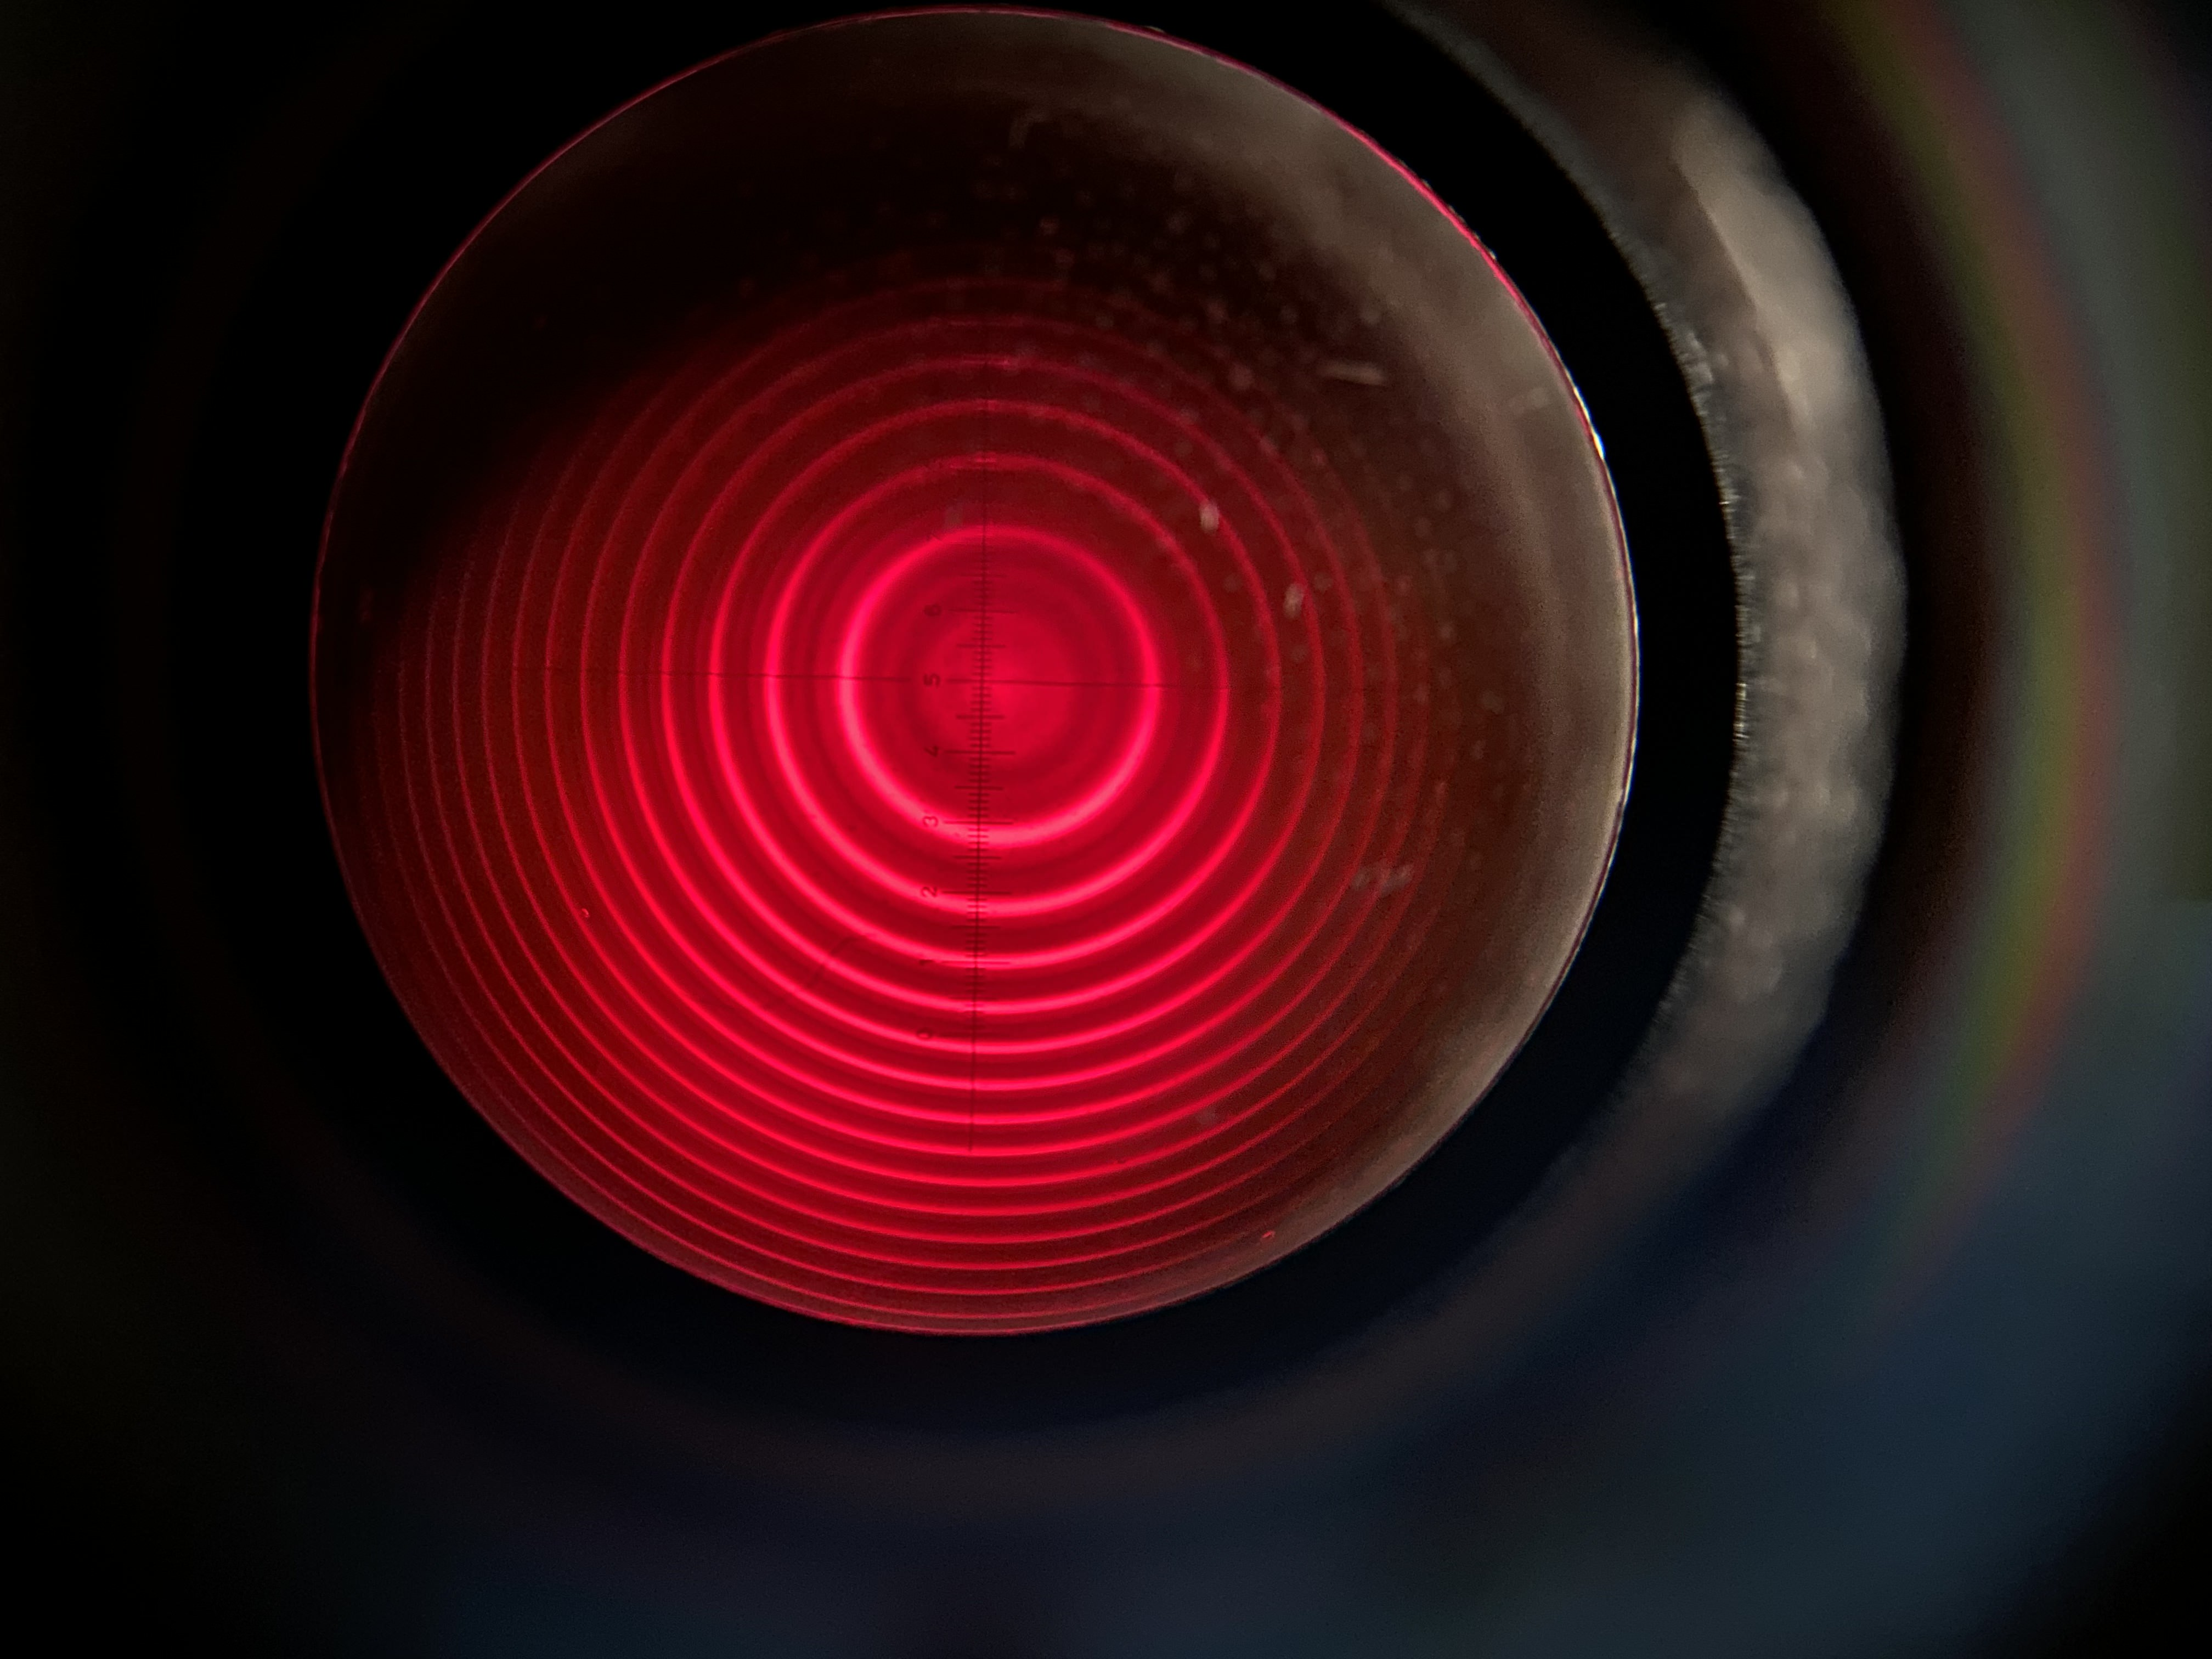
\includegraphics[width=.8\linewidth]{zeeman-longitudinal-mit-45}
  \caption{Interferenzmuster bei longitudinaler Beobachtung mit Magnetfeld, mit Polarisationsfilter.}
  \label{fig:zeeman-longitudinal-mit-45}
\end{figure}


\subsection{Messung des Zeeman-Effekts}
Es soll nun quantitativ die Stärke der Aufspaltung in Abhängigkeit des anliegenden Magnetfelds gemessen werden,
mit dem Ziel, das Bohrsche Magneton $\mu_B$ zu bestimmten.
Hierzu wird die transversale Konfiguration verwendet und $\lambda/4$-Platte sowie Polarisationsfilter aus dem Strahlengang entfernt.

\subsubsection{Magnetfeldkalibrierung}
Es wird die Abhängigkeit der Magnetfeldstärke vom fließenden Strom durchmessen, um daraus eine Kalibrierungskurve zu erstellen.
Hierzu wird anstatt der Cadmiumlampe eine Hall-Sonde genau mittig zwischen den Polschuhen eingeführt.
In Reihe zu den Magneten wird ein \enquote{Cassy-Modul} eingeschaltet,
wodurch am Computer mithilfe einer speziellen Software die Abhängigkeit automatisch aufgezeichnet werden kann.
Die Messung wird gestartet und der Strom allmählich bis zum maximal erreichbaren Wert hochgefahren.
Dann wird die Messung gestoppt und der Strom wieder ausgeschaltet.

Eine solche Kalibrierung wurde zweimal durchgeführt, einmal vor und einmal nach den Messungen aus \ref{messungmessung}.
In Abb. \ref{fig:magnetkalib} sind die Messdaten zusammen mit einem $\chi^2$-Fit der Form
\[
  B(I) = a + bI + cI^2 + dI^3
\]
dargestellt. Als Fehlerwerte auf $I$ und $B$ wurden dabei $2\%$ des jeweiligen Werts angesetzt,
wobei Fehlerwerte von $\SI{0.002}{\A}$ und $\SI{0.2}{\mT}$ nicht unterschritten werden dürfen.

\begin{figure}[H]
  \centering
  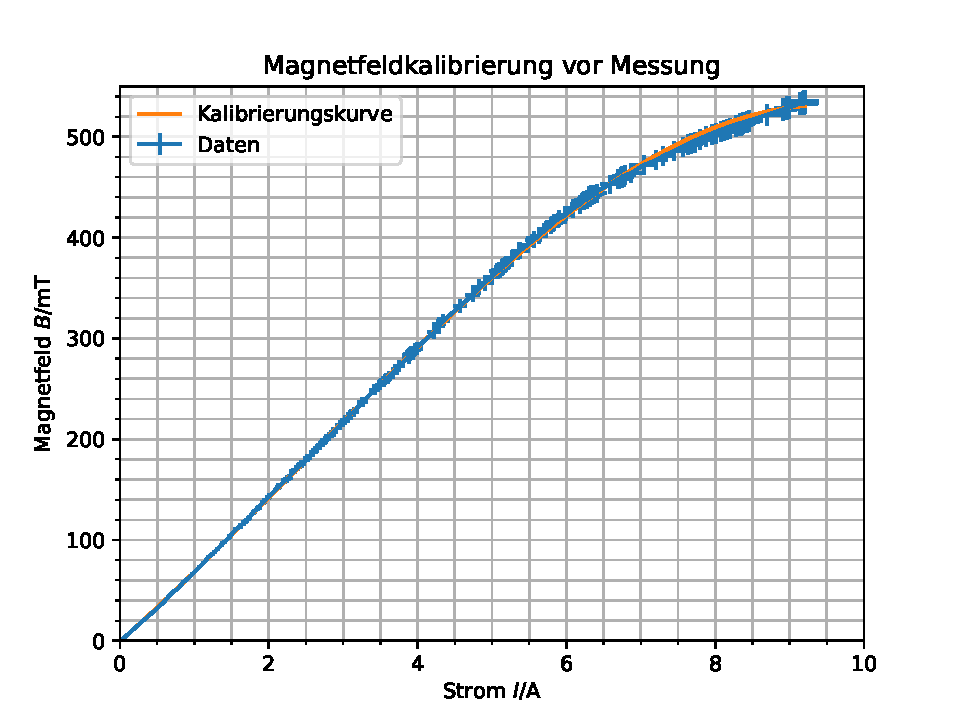
\includegraphics[width=.8\linewidth]{magnetkalib}
  \caption{Magnetfeldkalibierung vor der Messung mit CCD-Kamera}
  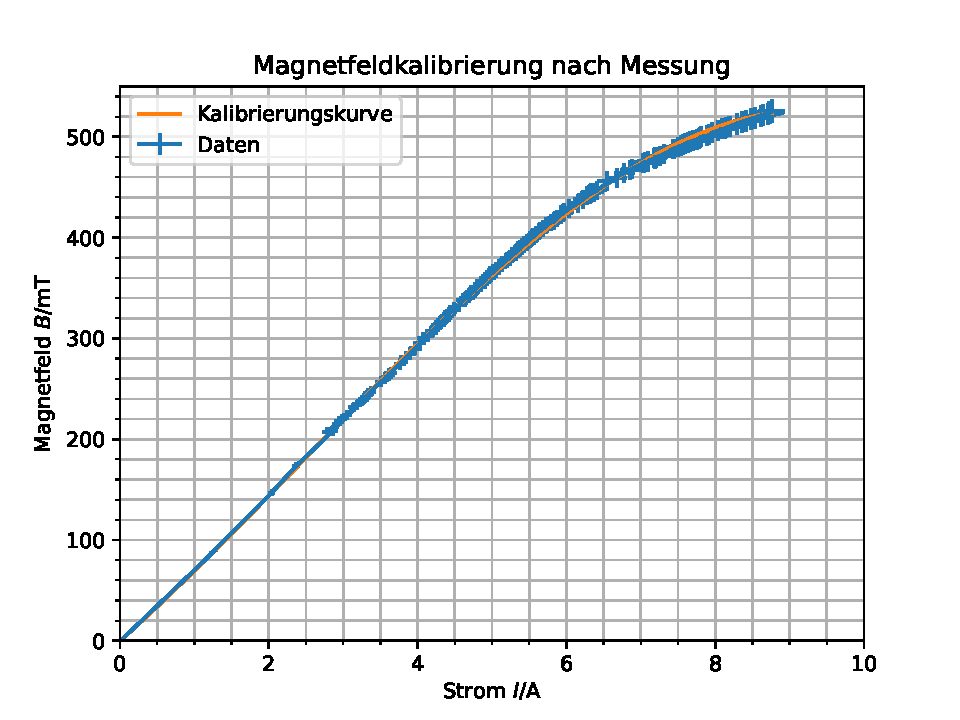
\includegraphics[width=.8\linewidth]{magnetkalib2}
  \caption{Magnetfeldkalibierung nach der Messung mit CCD-Kamera}
  \label{fig:magnetkalib}
\end{figure}

\begin{align*}
  a_1&=\SI{-0.548 \pm 0.025}{\mT},\ b_1=\SI{65.44 \pm 0.16}{\mT\per\A}, \\
  c_1&=\SI{3.96 \pm 0.065}{\mT\per\A\squared},\ d_1=\SI{-0.5213 \pm 0.0059}{\mT\per\A\cubed} \\
  a_1&=\SI{-0.104 \pm 0.027}{\mT},\ b_1=\SI{66.20 \pm 0.53}{\mT\per\A}, \\
  c_1&=\SI{3.97 \pm 0.186}{\mT\per\A\squared},\ d_1=\SI{-0.5361 \pm 0.0152}{\mT\per\A\cubed}
\end{align*}

Diese Werte sind in relativ guter Übereinstimmung miteinander; alle Parameter haben Überschneidungen in ihren Fehlerbereichen.
Leichte Abweichungen, z.B. beim Parameter $a$ lassen sich unter anderem dadurch erklären, dass die zweite Messung durchgeführt wurde,
als die Magnetspulen noch heiß vom vorigen Betrieb waren. Dies kann die Ergebnisse verändern.

Um eine einzelne Kalibrationskurve zu haben, verwenden wir im Folgenden die Mittelwerte der Parameter:
\begin{align*}
  % i = \frac{i_1+i_2}{2},\enspace \Delta I = \frac{\sqrt{i_1^2 + i_2^2}}{2}
  i &= \frac{i_1+i_2}{2},\enspace i=a,\,b,\,c,\,d \\
  a&=\SI{-0.326 \pm 0.019}{\mT},\ b=\SI{65.82 \pm 0.28}{\mT\per\A}, \\
  c&=\SI{3.96 \pm 0.099}{\mT\per\A\squared},\ d=\SI{-0.5288 \pm 0.0082}{\mT\per\A\cubed}
\end{align*}
Der Fehler wird dabei mithilfe von Gauß'scher Fehlerfortpflanzung bestimmt.


\subsubsection{Messungen mit CCD-Kamera} \label{messungmessung}
Die Messung der Positionen der Interferenzmaxima erfolgt mithilfe einer CCD-Kamera, die anstatt des Okulars
in den Strahlengang eingesetzt wird. Die Kamera (Auflösung von $1024$ Pixeln) wird mit dem Computer verbunden, wo mithilfe eines dafür ausgelegten
Programms die Lichtintensität in Abhängigkeit des Ablenkwinkels $\alpha$ aufgenommen wird.
Dabei wird $\alpha$ automatisch aus der Pixel-Position $p$ berechnet nach der Formel
\[
  \alpha = \arctan(\frac{(1024-p) \cdot \SI{0.014}{\mm}}{f}),\ f=\SI{150}{\mm}\ (\cite{Anleitung}, S.7)
\]
\todo{braucht man Seitenangaben?}

Nun wird das Magnetfeld durch Änderung des Stroms variiert und am Computer beobachtet,
wie sich die Aufspaltung der Linien verändert.
Für $10$ verschiedene Ströme wird die Messung (Werte der Intensität $I$ in Abhängigkeit des Winkels $\alpha$) jeweils abgespeichert.
Aus jeder Messung wird eine Beugungsordnung ausgesucht, bei der wir die Positionen drei verschiedenen Peaks bestimmen.
Dazu wird immer nur der Bereich dieser drei Peaks aus den Daten ausgewählt und ein Fit der Form
% Dies erfolgt mithilfe eines Dreifachen Gauß-Fits der Form
\[
  I(\alpha) = B + G(\alpha; a_1, \mu_1, \sigma_1) + G(\alpha; a_2, \mu_2, \sigma_2) + G(\alpha; a_3, \mu_3, \sigma_3)
\]
mit drei Überlagerten verallgemeinerten Gauß-Funktionen
\[
  G(xg a, \mu, \sigma) = a \exp(\frac{(x-b)^2}{2c^2})
\]
durchgeführt. Der additive Parameter $B$ ermöglicht die Berücksichtigung einer eventuell vorhanden gleichmäßigen Grundausleuchtung
und sorgt nach visueller Inspektion erfahrungsgemäß für bessere Anpassung der Gauß-Parameter an die Daten.


\clearpage
\section{Franck-Hertz-Versuch}
Im folgenden Abschnitt wird das Franck-Hertz-Experiment durchgeführt und anschließend detailliert 
diskutiert. Anhand der durch das Cassy-Modul gemessenen Anodenstromkurven \( I_A \) wird die 
Energiedifferenz \( \Delta E \) zwischen den Energieniveaus des Quecksilbers $Hg$, \( 6S \) und \( 6P \), 
präzise bestimmt.
\subsection{Aufbau}
In einer Franck-Hertz-Röhre, die mit Quecksilbers gefüllt ist, befindet sich eine glühende 
Kathode mit einer Heisspannung $U_H$, die die Elektronen durch thermische Emmission freisetzt und in der 
Richtung einer positiv geladenen Anode beschleunigt. Die Beschleunigungsspannung $U_B$ zwischen Kathode 
und Anode bestimmt die kinetische Energie der Elektronen, bevor sie auf die Quecksilberatome treffen.

Zwischen der Kathode und der Anode befindet sich ein Gitter, das in einigen Konstruktionen mit einem kleinen 
Gegenfeld ausgestattet ist, um Elektronen, die nach elastische nd inelastische Stößen ihre kinetische Energie 
verloren haben, daran zu hindern, die Anode zu erreichen. Der Anodenstrom $I_A$
wird dann in Abhängigkeit von der Spannung $U_B$ gemessen. Bei bestimmten Spannungswerten zeigt der Anodenstrom charakteristische Einbrüche, die auftreten, wenn die Elektronen genau die Energie erreichen, die nötig ist, um ein Quecksilberatom vom Grundzustand (6S) in einen angeregten Zustand (6P) zu heben.
 Durch diesen inelastischen Stoß verlieren die Elektronen ihre kinetische Energie und tragen dadurch nicht mehr zum Stromfluss bei.

Die Spannungsdifferenz zwischen aufeinanderfolgenden Strommaxima liefert die Energie $\Delta E$, die den 
Übergang zwischen den 6S- und 6P-Niveaus beschreibt. 
\subsection{Durchführung und Auswertung}
Zunächst wird die Energiedifferenz $\Delta E$ zwischen die Energieniveaus des $Hg$ bestimmt. 
Dabei sollen die Breiten der Kurven bzw. die Peaks bestimmt werden. Dazu werden Gaußkurven an die Daten angepasst,
die mithilfe des Programms \textit{Fityk} gemacht werden.
\\ Es ist zu beachten, dass bei den verschiedenen Messungen nicht dieselbe Anzahl an Peaks 
erfasst wurde. Daher wurden nur die erkennbaren Peaks analysiert und in die Tabellen 
aufgenommen. 
\subsection*{Fityk Version 1.3.1}
In \textit{Fityk} werden Gauß-Fits durch Auswahl eines Datenbereichs und Anwendung einer Gaußfunktion als 
Modell durchgeführt. Die Gaußfunktion hat die Form 

\begin{equation*}
f(x) = a \cdot e^{-\frac{(x - \mu)^2}{2 \sigma^2}}
\end{equation*}
wobei $a$ die Amplitude, $\mu$ der Mittelwert (Zentrum des Peaks) und $\sigma$ die Standardabweichung 
ist. Das Programm optimiert die Parameter $a$, $\mu$ und $\sigma$, sodass die Abweichung zwischen dem Modell 
und den Datenpunkten minimiert wird. Die Methode der kleinsten Quadrate wird oft verwendet, um den
 Fehlerausdruck
\begin{equation*}
\sum_{i=1}^{N} (y_i - f(x_i))^2
\end{equation*}
zu minimieren, wobei $y_i$ die gemessenen Datenpunkte und $f(x_i)$ die entsprechenden Werte der Gaußfunktion 
sind. Dadurch entsteht eine Gaußkurve, die die Daten im ausgewählten Bereich bestmöglich beschreibt.
\subsection*{Diskussion der Daten}
 Wie bereits erwähnt, wurde während des Experiments nicht dieselbe Anzahl von Peaks erfasst. Dies stellt jedoch 
 kein Problem dar, da eine ausreichende Anzahl an Messwerten vorliegt. Zudem wurde in \textit{Fityk} eine 
 Hintergrundfunktion zu den Gauß-Fits hinzugefügt, sodass die Gesamtsumme der Gauß-Peaks eine bessere 
 Übereinstimmung mit den im Experiment beobachteten Peaks aufweist. Unter Berücksichtigung der oben genannten Anpassungen 
 und Messmethoden folgen nun die entsprechenden Graphen. 
\begin{figure}[H]
  \centering
  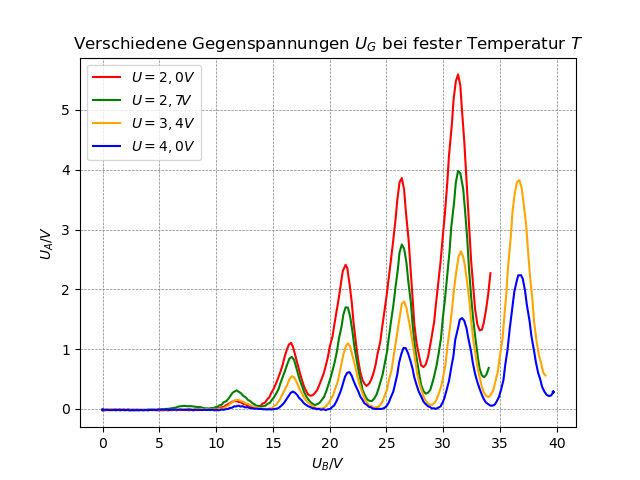
\includegraphics[scale=0.55]{FH_vieleT.png}
  \caption{Die gemessene Beschleunigungsspannung $U_B$ gegen Anodenspannung $U_A$ bei
   verschiedene Gegenspannung $T$ und fester Temperatur $U_G$}
\end{figure}
\clearpage

\begin{figure}[H]
  \centering
  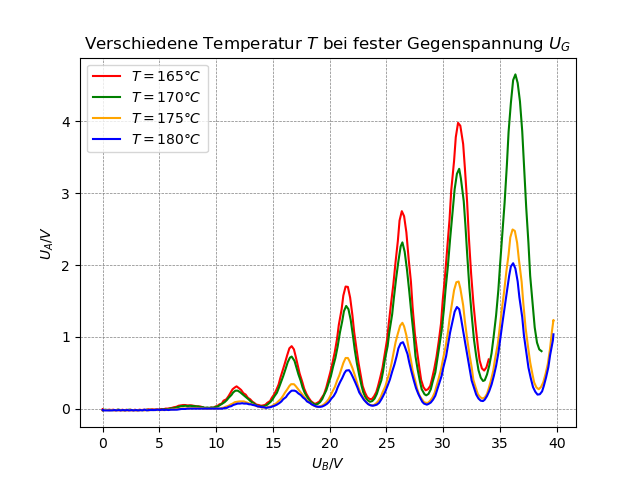
\includegraphics[scale=0.55]{FH_vieleU.png}
  \caption{Die gemessene Beschleunigungsspannung $U_B$ gegen Anodenspannung $U_A$ 
  verschiedenen Temperaturen $T$ und Gegenspannung $U_G$}
\end{figure}

\subsection*{Bestimmung der $\Delta$Energiedifferenz}
Um die Eindeutigkeit zu gewährleisten, bezeichnen wir die Peaks bzw. die Erwartungswerte mit $U^i_B$ und 
fassen alle relevanten Informationen in einer Tabelle zusammen.
Der Fehler des Mittelwerts wird durch die folgende Formel und in der Tabelle dargestellt:
\begin{equation*}
\Delta(U^i_B) = \sqrt{\frac{1}{N} \sum_{n=1}^{N} \left( \delta U_{i,n}^B \right)^2}
\end{equation*}
Dabei ist \( N \) die Anzahl der Werte, die zur Berechnung des Mittelwerts beitragen.

Im Folgenden sind die Mittelwerte der Beschleunigungsspannung sowie die entsprechenden Fehler dargestellt.
\begin{table}[H]
  \centering
  \begin{tabular}{cc} 
      \hline
      & Mittelwert [V] \\ \hline
      $U^1_B$ & 36.3 \\ \hline
      $U^2_B$ & 31.2 \\ \hline
      $U^3_B$ & 26.3 \\ \hline
      $U^4_B$ & 21.6 \\ \hline
      $U^5_B$ & 16.6 \\ \hline
      $U^6_B$ & 11.8 \\ \hline
  \end{tabular}
  \caption{Mittelwerte zu $U^i_B$}
  \label{tab:median_values}
\end{table}

\begin{table}[H]
  \centering
  \begin{tabular}{cc} 
      \hline
       & Mittelwert [V] \\ \hline
      $\delta U^1_B$ & $\pm 0.0504$ \\ \hline
      $\delta U^2_B$ & $\pm 0.133$ \\ \hline
      $\delta U^3_B$ & $\pm 0.0112$ \\ \hline
      $\delta U^4_B$ & $\pm 0.0161$ \\ \hline
      $\delta U^5_B$ & $\pm 0.0307$ \\ \hline
      $\delta U^6_B$ & $\pm 0.131$ \\ \hline
  \end{tabular}
  \caption{Mittelwerte zu $\delta U^i_B$}
  \label{tab:mean_values}
\end{table}
Nun kann man aus den Diferenzen der benachbaren Peaks der Energiedifferenz $\Delta E$ bestimmt werden. 
\begin{equation*}
  \Delta E=(4.9 \pm 0.0803)eV
\end{equation*}
Das Ergebnis unserer experimentellen Messungen ist äußerst erfreulich und stimmt vollständig 
mit dem erwarteten theoretischen Wert der Übergang zwischen $6^1 S_o \rightarrow 6^3P_1$ überein. 
Wie man in der Abbildung sich anschauen kann. 
\begin{figure}[H]
  \centering
  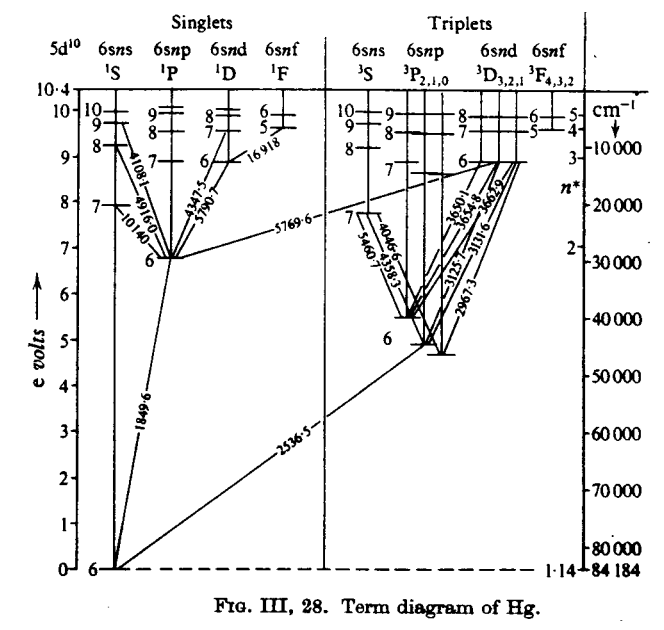
\includegraphics[scale=0.45]{Vereinfachtes Hg-Termschema.png}
  \caption{Termschema des Quecksilbers}
\end{figure}
\clearpage
\subsection{Einfluss der Temperatur $T$ und der Gegenspannung $U_2$}

Untersucht man den Zusammenhang zwischen Energiedifferenz und Wirkungsquerschnitt, so 
stellt man fest, dass die Wechselwirkung ihr Maximum bei $\Delta E = 4{.}9 \, \mathrm{eV}$ 
erreicht. Dennoch weist der Peak eine Breite auf, was auf die Natur des Triplet-Zustands 
$6^3P$ zurückzuführen ist, da einige Elektronen mit etwas geringerer oder höherer Energie 
wechselwirken können.(siehe Abbildung \ref{Wirkungsquerschnitt})

Zudem erkennt man mithilfe des Anhangs im Praktikumskript, dass der Dampfdruck von 
Quecksilber stark von der Temperatur abhängt (siehe untenstehende Formel).

\begin{equation*}
  log(p) = 10.55 - \frac{3333}{T} - 0.85log(T)
\end{equation*}
Daraus folgt, dass bei steigender Temperatur vermehrt thermische Stöße zwischen den H
g-Atomen stattfinden können, was dazu führt, dass weniger Elektronen die notwendige 
Energie besitzen, um die Anode zu erreichen. Andererseits treten bei niedrigeren 
Temperaturen weniger Stöße auf, was zur Folge hat, dass nur geringe oder gar keine Peaks 
beobachtet werden können.


\begin{figure}[H]
  \centering
  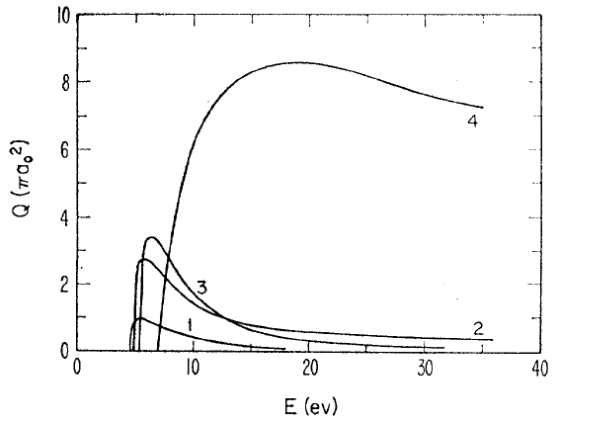
\includegraphics[scale=0.55]{Totaler Wirkungsquerschnitt.png}
  \caption{Totaler Wirkungsquerschnitt $Q(\pi a^2_0$) von Hg für Elektronenstoßanregung}
  \label{Wirkungsquerschnitt}
\end{figure}
\clearpage
\section{Fazit}

Im zweiten Versuchsteil wird der Franck-Hertz-Versuch aufgebaut und untersucht. Dabei 
wird die Beschleunigungsspannung in Abhängigkeit von der Anodenspannung bei verschiedenen 
Temperaturen und Gegenspannungen aufgezeichnet, wodurch die erwarteten Peaks entstehen. 
Mithilfe der Berechnung des Erwartungswerts $\mu_i$ und der Standardabweichung $\sigma_i$ 
wird nach der Datenanalyse festgestellt, dass die Energiedifferenz für den Übergang im 
Hg-Atom zwischen den Zuständen $6^1S_0$ und $6^3P_1$ den Wert $\Delta E = (4.9 \pm 0.0803) \, 
\text{eV}$ annimmt, was erstaunlich gut mit dem theoretischen Wert übereinstimmt. Zudem 
fällt auf, dass bei erhöhter Temperatur $T$ und Gegenspannung $U_G$ die Anodenspannung $U_A$ abnimmt.



\clearpage
\begin{thebibliography}{9}

\bibitem{Anleitung}
\textit{Physikalisches Praktikum Teil IV -- Versuchsbeschreibungen}, Universität Bonn, Abruf 29.10.2024

\bibitem{Leybold}
\textit{Beobachtung des normalen Zeeman-Effekts in transversaler und longitudinaler Konfiguration}, Leybold Didactic, Abruf 30.10.2024

\end{thebibliography}
\clearpage
\section{Anhang}
\begin{table}[H]
  \centering
  \begin{tabular}{|c|c|c|}
      \hline
      Parameter & Wert & Fehler $\Delta$ \\ \hline
      $\mu_1$ & 31.1 & $\pm$ 0.0183 \\ \hline
      $\sigma_1$& 1.26 & $\pm$ 0.0358 \\ \hline
      $\mu_2$ & 26.1 & $\pm$ 0.0162 \\ \hline
      $\sigma_2$ & 1.08 & $\pm$ 0.0249 \\ \hline
      $\mu_3$ & 21.2 & $\pm$ 0.024 \\ \hline
      $\sigma_3$ & 0.91 & $\pm$ 0.0298 \\ \hline
      $\mu_4$ & 16.4 & $\pm$ 0.0365 \\ \hline
      $\sigma_4$ & 0.843 & $\pm$ 0.0522 \\ \hline
      $\mu_5$ & 11.7 & $\pm$ 0.237 \\ \hline
      $\sigma_5$ & 0.669 & $\pm$ 0.306 \\ \hline
  \end{tabular}
  \caption{Parameter bei $U_G=2.0V$ und $T=165^\circ C$}
  \label{tab:data_no_height}
\end{table}
\begin{table}[H]
  \centering
  \begin{tabular}{|c|c|c|}
      \hline
      Parameter & Wert & Fehler $\Delta$ \\ \hline
      $\mu_1$ & 31.3 & $\pm$ 0.00925 \\ \hline
      $\sigma_1$ & 1.04 & $\pm$ 0.0129 \\ \hline
      $\mu_2$ & 26.3 & $\pm$ 0.00979 \\ \hline
      $\sigma_2$ & 0.967 & $\pm$ 0.0151 \\ \hline
      $\mu_3$ & 21.4 & $\pm$ 0.0133 \\ \hline
      $\sigma_3$ & 0.914 & $\pm$ 0.019 \\ \hline
      $\mu_4$ & 16.6 & $\pm$ 0.0242 \\ \hline
      $\sigma_4$ & 0.885 & $\pm$ 0.0321 \\ \hline
      $\mu_5$ & 11.9 & $\pm$ 0.0715 \\ \hline
      $\sigma_5$ & 0.884 & $\pm$ 0.0916 \\ \hline
  \end{tabular}
  \caption{Parameter bei $U_G=2.7V$ und $T=165^\circ C$}
  \label{tab:data_no_height_2}
\end{table}

\begin{table}[H]
  \centering
  \begin{tabular}{|c|c|c|}
      \hline
      Parameter & Wert & Fehler $\Delta$ \\ \hline
      $\mu_1$ & 36.7 & $\pm$ 0.00818 \\ \hline
      $\sigma_1$ & 1.19 & $\pm$ 0.00971 \\ \hline
      $\mu_2$ & 31.6 & $\pm$ 0.0125 \\ \hline
      $\sigma_2$ & 1.02 & $\pm$ 0.0153 \\ \hline
      $\mu_3$ & 26.5 & $\pm$ 0.0121 \\ \hline
      $\sigma_3$ & 0.95 & $\pm$ 0.0143 \\ \hline
      $\mu_4$ & 21.6 & $\pm$ 0.0181 \\ \hline
      $\sigma_4$ & 0.871 & $\pm$ 0.0215 \\ \hline
      $\mu_5$ & 16.7 & $\pm$ 0.0362 \\ \hline
      $\sigma_5$ & 0.846 & $\pm$ 0.0423 \\ \hline
  \end{tabular}
  \caption{Parameter bei $U_G=3.4V$ und $T=165^\circ C$}
  \label{tab:data_no_height_3}
\end{table}

\begin{table}[H]
  \centering
  \begin{tabular}{|c|c|c|}
      \hline
      Parameter & Wert & Fehler $\Delta$ \\ \hline
      $\mu_1$ & 36.8 & $\pm$ 0.00835 \\ \hline
      $\sigma_1$ & 1.0 & $\pm$ 0.0123 \\ \hline
      $\mu_2$ & 31.7 & $\pm$ 0.00744 \\ \hline
      $\sigma_2$ & 0.944 & $\pm$ 0.00934 \\ \hline
      $\mu_3$ & 26.7 & $\pm$ 0.00927 \\ \hline
      $\sigma_3$ & 0.837 & $\pm$ 0.0111 \\ \hline
      $\mu_4$ & 21.7 & $\pm$ 0.0151 \\ \hline
      $\sigma_4$ & 0.769 & $\pm$ 0.0178 \\ \hline
      $\mu_5$ & 16.8 & $\pm$ 0.0313 \\ \hline
      $\sigma_5$ & 0.712 & $\pm$ 0.0371 \\ \hline
  \end{tabular}
  \caption{Parameter bei $U_G=4.0V$ und $T=165^\circ C$}
  \label{tab:data_no_height_5}
\end{table}

\begin{table}[H]
  \centering
  \begin{tabular}{|c|c|c|}
      \hline
      Parameter & Wert & Fehler $\Delta$ \\ \hline
      $\mu_1$ & 36.3 & $\pm$ 0.00915 \\ \hline
      $\sigma_1$ & 1.11 & $\pm$ 0.0139 \\ \hline
      $\mu_2$ & 31.2 & $\pm$ 0.00858 \\ \hline
      $\sigma_2$ & 1.02 & $\pm$ 0.0136 \\ \hline
      $\mu_3$ & 26.3 & $\pm$ 0.0105 \\ \hline
      $\sigma_3$ & 0.966 & $\pm$ 0.0152 \\ \hline
      $\mu_4$ & 21.4 & $\pm$ 0.0148 \\ \hline
      $\sigma_4$ & 0.92 & $\pm$ 0.0205 \\ \hline
      $\mu_5$ & 16.6 & $\pm$ 0.0277 \\ \hline
      $\sigma_5$ & 0.889 & $\pm$ 0.0364 \\ \hline
      $\mu_6$ & 11.9 & $\pm$ 0.0832 \\ \hline
      $\sigma_6$ & 0.893 & $\pm$ 0.106 \\ \hline
  \end{tabular}
  \caption{Parameter bei $U_G=2.7V$ und $T=170^\circ C$}
  \label{tab:data_no_height_6}
\end{table}

\begin{table}[H]
  \centering
  \begin{tabular}{|c|c|c|}
      \hline
      Parameter & Wert & Fehler  \\ \hline
      $\mu_1$ & 36.3 & $\pm$ 0.128 \\ \hline
      $\sigma_1$ & 1.67 & $\pm$ 0.212 \\ \hline
      $\mu_2$ & 30.8 & $\pm$ 0.734 \\ \hline
      $\sigma_2$ & 1.08 & $\pm$ 0.26 \\ \hline
      $\mu_3$ & 26.3 & $\pm$ 0.0108 \\ \hline
      $\sigma_3$ & 0.929 & $\pm$ 0.0138 \\ \hline
      $\mu_4$ & 21.5 & $\pm$ 0.0112 \\ \hline
      $\sigma_4$ & 0.981 & $\pm$ 0.0135 \\ \hline
      $\mu_5$ & 16.8 & $\pm$ 0.0232 \\ \hline
      $\sigma_5$ & 1.00 & $\pm$ 0.0275 \\ \hline
  \end{tabular}
  \caption{Parameter bei $U_G=2.7V$ und $T=175^\circ C$}
  \label{tab:data_no_height_7}
\end{table}

\begin{table}[H]
  \centering
  \begin{tabular}{|c|c|c|}
      \hline
      Parameter & Wert & Fehler  \\ \hline
      $\mu_1$ & 36.1 & $\pm$ 0.00659 \\ \hline
      $\sigma_1$ & 0.952 & $\pm$ 0.0118 \\ \hline
      $\mu_2$ & 31.2 & $\pm$ 0.00694 \\ \hline
      $\sigma_2$ & 0.968 & $\pm$ 0.0108 \\ \hline
      $\mu_3$ & 26.3 & $\pm$ 0.0095 \\ \hline
      $\sigma_3$ & 0.921 & $\pm$ 0.0152 \\ \hline
      $\mu_4$ & 21.6 & $\pm$ 0.016 \\ \hline
      $\sigma_4$ & 0.893 & $\pm$ 0.0233 \\ \hline
      $\mu_5$ & 16.8 & $\pm$ 0.0351 \\ \hline
      $\sigma_5$ & 0.911 & $\pm$ 0.0544 \\ \hline
  \end{tabular}
  \caption{Parameter bei $U_G=2.7V$ und $T=180^\circ C$}
  \label{tab:data_no_height_8}
\end{table}

\begin{table}[H]
  \centering
  \begin{tabular}{cccccc} 
      \hline
      $U^1_B$[V] & $U^2_B$[V] & $U^3_B$[V] & $U^4_B$[V] & $U^5_B$[V] & $U^6_B$[V] \\ \hline
      36.7 & 31.1 & 26.1 & 21.2 & 16.4 & 11.7 \\ \hline
      36.8 & 31.3 & 26.3 & 21.4 & 16.6 & 11.9 \\ \hline
      36.3 & 31.6 & 26.5 & 21.6 & 16.7 & 11.9 \\ \hline
      36.3 & 31.7 & 26.7 & 21.7 & 16.6 & - \\ \hline
      36.1 & 31.2 & 26.3 & 21.4 & 16.8 & - \\ \hline
      - & 30.8 & 26.3 & 21.5 & 16.8 & - \\ \hline
      - & 31.2 & 26.3 & 21.6 & 16.8 & - \\ \hline
  \end{tabular}
  \caption{zugeordnete $U^i_B$}
  \label{tab:measurements}
\end{table}

\begin{table}[H]
  \centering
  \small 
  \begin{tabular}{cccccc} 
      \hline
      $\delta U^1_B$[V] & $\delta U^2_B$[V] & $\delta U^3_B$[V] & $\delta U^4_B$[V] & $\delta U^5_B$[V] & $U^6_B$[V] \\ \hline
      $\pm 0.00818$ & $\pm 0.0183$ & $\pm 0.0162$ & $\pm 0.024$ & $\pm 0.0365$ & $\pm 0.237$ \\ \hline
      $\pm 0.00835$ & $\pm 0.00925$ & $\pm 0.00979$ & $\pm 0.0133$ & $\pm 0.0242$ & $\pm 0.0715$ \\ \hline
      $\pm 0.00915$ & $\pm 0.0125$ & $\pm 0.0121$ & $\pm 0.0181$ & $\pm 0.0362$ & $\pm 0.0832$ \\ \hline
      $\pm 0.128$ & $\pm 0.00744$ & $\pm 0.00927$ & $\pm 0.0151$ & $\pm 0.0313$ & - \\ \hline
      $\pm 0.00659$ & $\pm 0.00858$ & $\pm 0.0105$ & $\pm 0.0148$ & $\pm 0.0277$ & - \\ \hline
      - & $\pm 0.734$ & $\pm 0.0108$ & $\pm 0.0112 $ & $\pm 0.0232$ & - \\ \hline
      - & $\pm 0.00694$ & $\pm 0.0095$ & $\pm 0.016$ & $\pm 0.0351$ & - \\ \hline
  \end{tabular}
  \caption{zugeordnete $\delta U^i_B$}
  \label{tab:measurements}
\end{table}
Im Folgenden sind die Mittelwerte der Beschleunigungsspannung sowie die entsprechenden Fehler dargestellt.
\begin{table}[H]
  \centering
  \begin{tabular}{cc} 
      \hline
      & Mittelwert [V] \\ \hline
      $U^1_B$ & 36.3 \\ \hline
      $U^2_B$ & 31.2 \\ \hline
      $U^3_B$ & 26.3 \\ \hline
      $U^4_B$ & 21.6 \\ \hline
      $U^5_B$ & 16.6 \\ \hline
      $U^6_B$ & 11.8 \\ \hline
  \end{tabular}
  \caption{Mittelwerte zu $U^i_B$}
  \label{tab:median_values}
\end{table}

\begin{table}[H]
  \centering
  \begin{tabular}{cc} 
      \hline
       & Mittelwert [V] \\ \hline
      $\delta U^1_B$ & $\pm 0.0504$ \\ \hline
      $\delta U^2_B$ & $\pm 0.133$ \\ \hline
      $\delta U^3_B$ & $\pm 0.0112$ \\ \hline
      $\delta U^4_B$ & $\pm 0.0161$ \\ \hline
      $\delta U^5_B$ & $\pm 0.0307$ \\ \hline
      $\delta U^6_B$ & $\pm 0.131$ \\ \hline
  \end{tabular}
  \caption{Mittelwerte zu $\delta U^i_B$}
  \label{tab:mean_values}
\end{table}
Nun kann man aus den Diferenzen der benachbaren Peaks der Energiedifferenz $\Delta E$ bestimmt werden. 
\begin{equation*}
  \Delta E=(4.9 \pm 0.0803)eV
\end{equation*}
Das Ergebnis unserer experimentellen Messungen ist äußerst erfreulich und stimmt vollständig 
mit dem erwarteten theoretischen Wert der Übergang zwischen $6^1 S_o \rightarrow 6^3P_1$ überein. 
Wie man in der Abbildung sich anschauen kann. 
\begin{figure}[H]
  \centering
  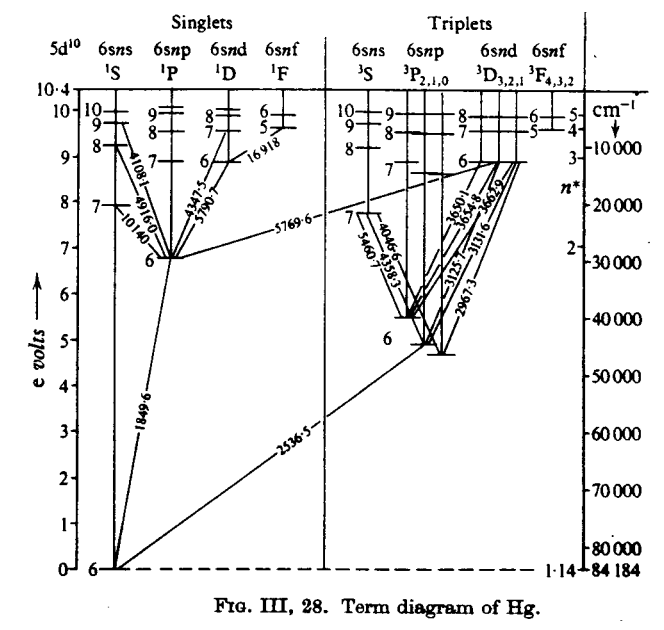
\includegraphics[scale=0.45]{Vereinfachtes Hg-Termschema.png}
  \caption{Termschema des Quecksilbers}
\end{figure}
\subsection{Einfluss der Temperatur $T$ und der Gegenspannung $U_2$}
\begin{figure}[H]
  \centering
  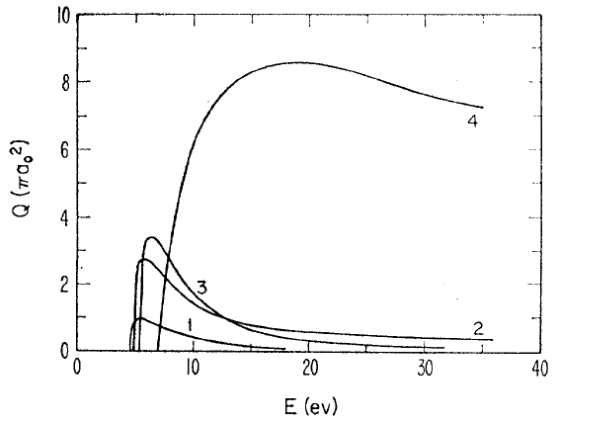
\includegraphics[scale=0.55]{Totaler Wirkungsquerschnitt.png}
  \caption{Totaler Wirkungsquerschnitt $Q(\pi a^2_0$) von Hg für Elektronenstoßanregung}
\end{figure}



\section{Fazit}
\end{multicols}
\clearpage

\section*{Anhang}

\begin{figure}[h]
  \centering
  \begin{minipage}{.49\linewidth}
    \centering
    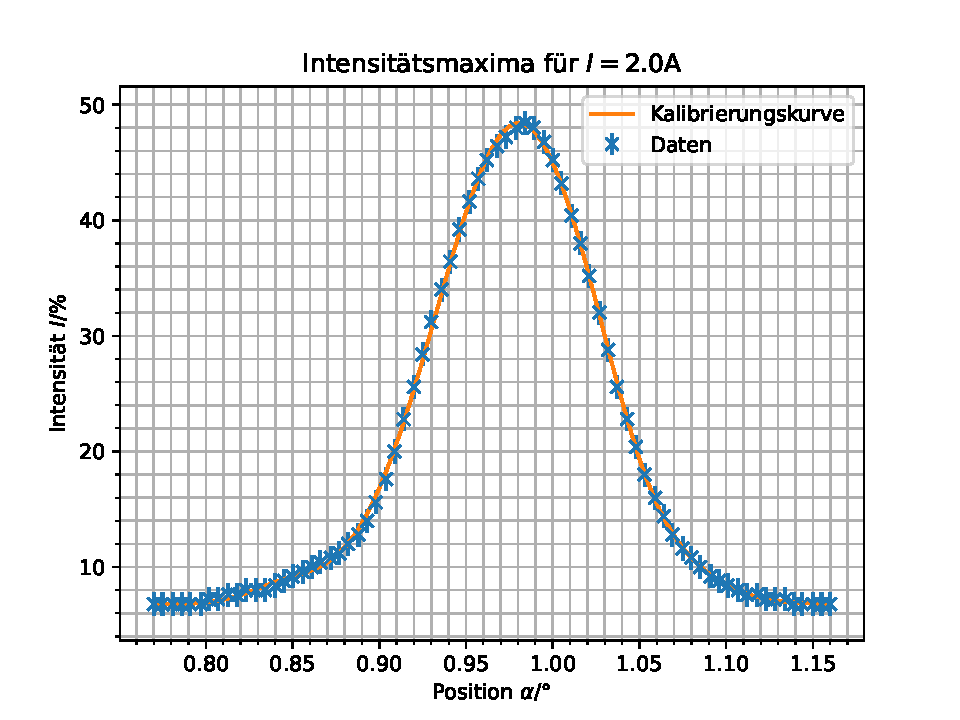
\includegraphics[width=\linewidth]{gauss_2.0A.pdf}
  \end{minipage}
  \hfill
  \begin{minipage}{.49\linewidth}
    \centering
    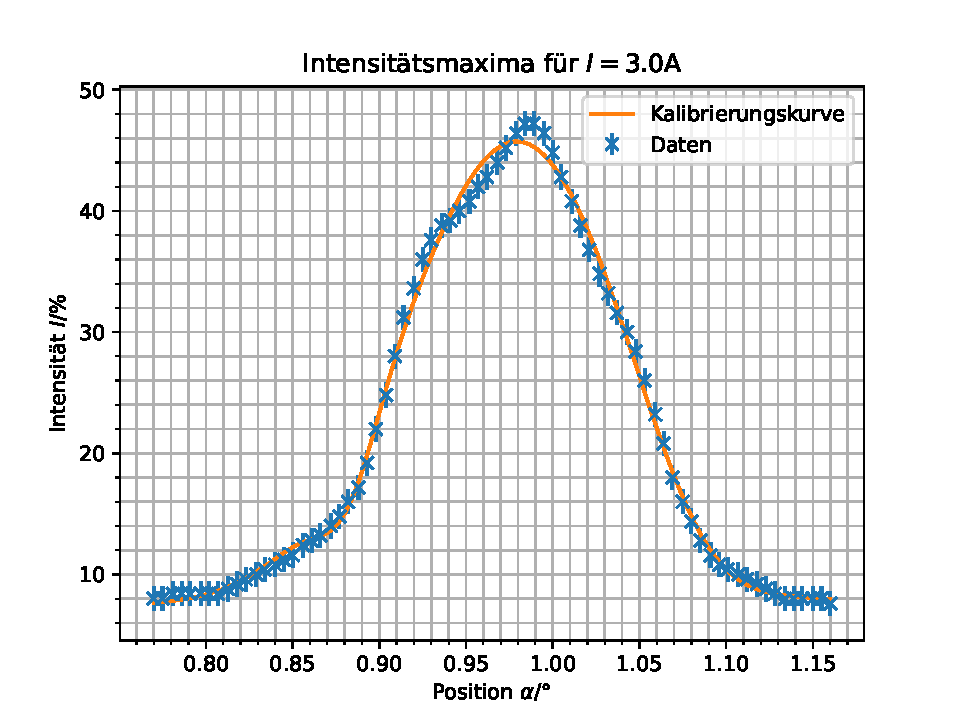
\includegraphics[width=\linewidth]{gauss_3.0A.pdf}
  \end{minipage}

  \begin{minipage}{.49\linewidth}
    \centering
    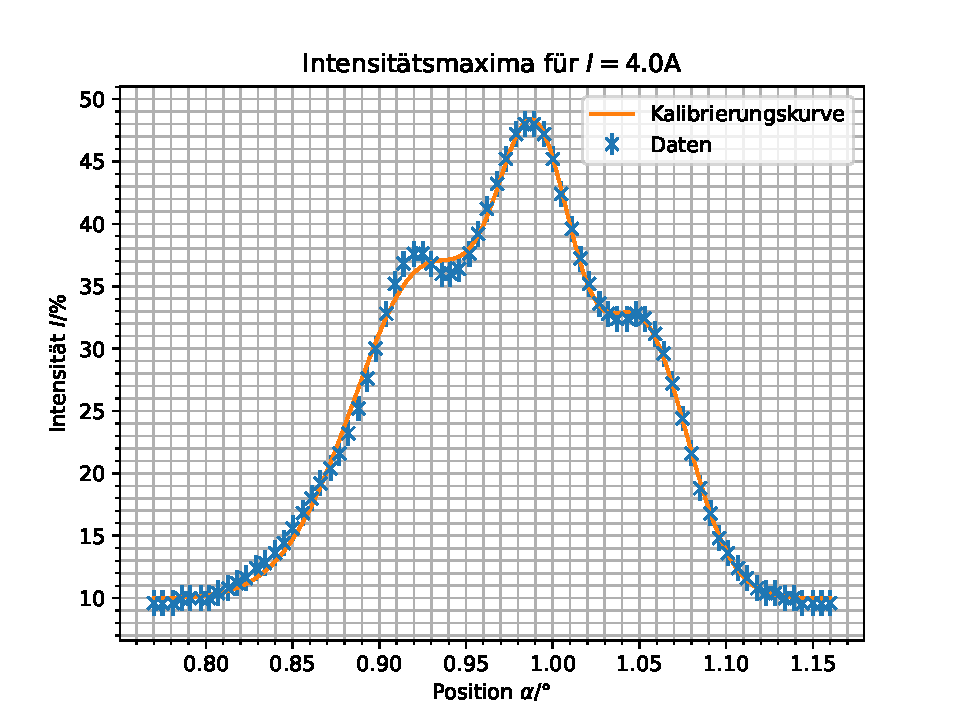
\includegraphics[width=\linewidth]{gauss_4.0A.pdf}
  \end{minipage}
  \hfill
  \begin{minipage}{.49\linewidth}
    \centering
    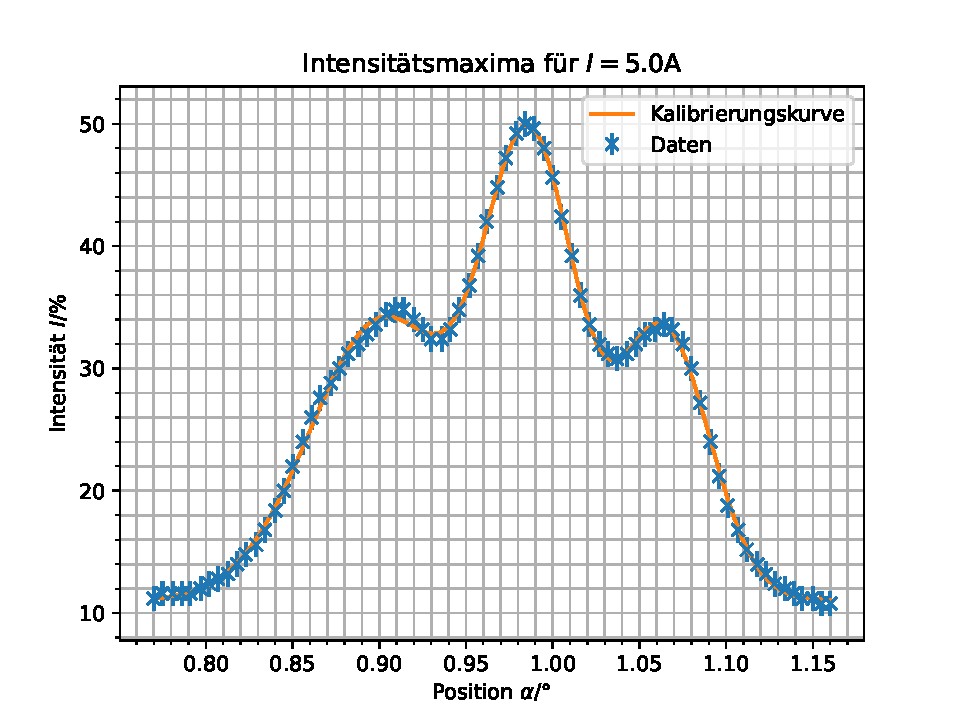
\includegraphics[width=\linewidth]{gauss_5.0A.pdf}
  \end{minipage}

  \begin{minipage}{.49\linewidth}
    \centering
    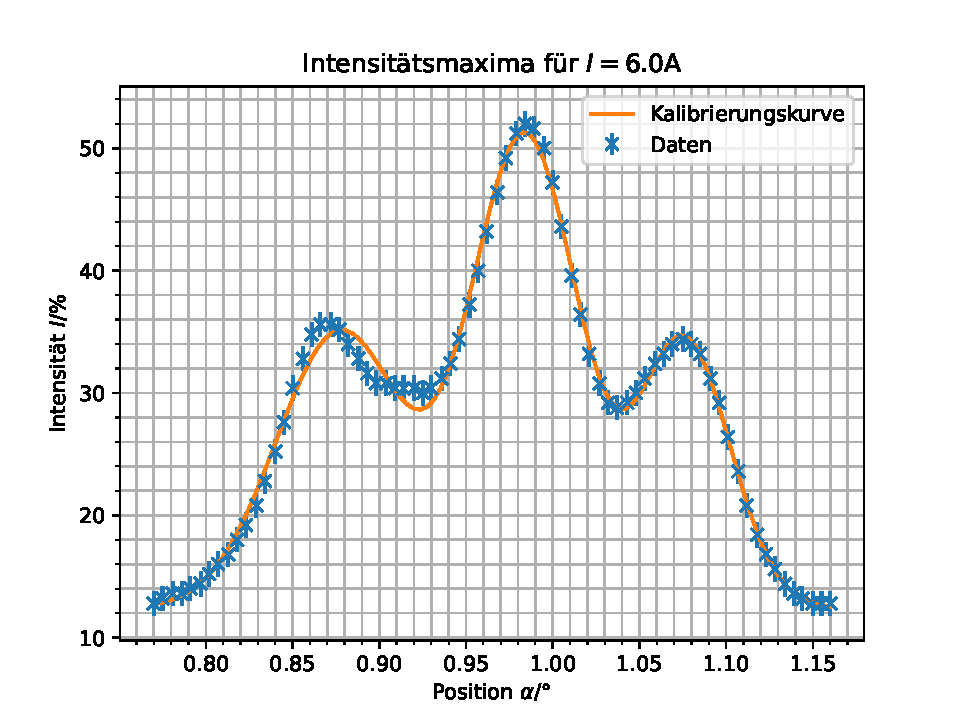
\includegraphics[width=\linewidth]{gauss_6.0A.pdf}
  \end{minipage}
  \hfill
  \begin{minipage}{.49\linewidth}
    \centering
    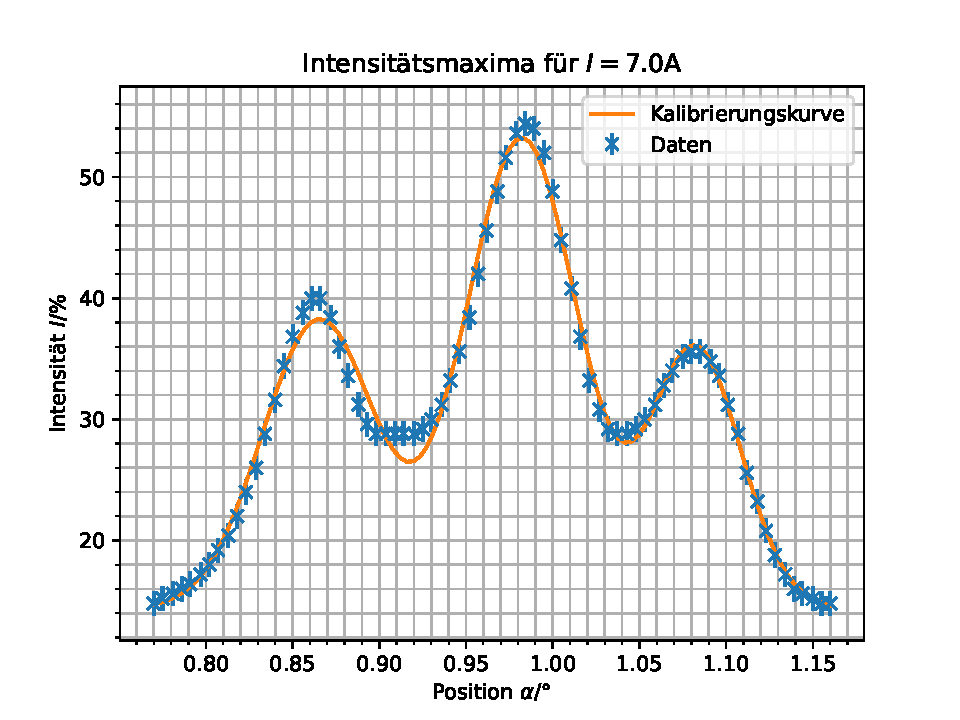
\includegraphics[width=\linewidth]{gauss_7.0A.pdf}
  \end{minipage}
  \caption{Ausgewählte Intensitätsmaxima für verschiedene Magnetströme $I$, mit Gauß-Fit [Teil 1]}
  \label{fig:gauss-fit-1}
\end{figure}

\begin{figure}[h]
  \centering
  \begin{minipage}{.49\linewidth}
    \centering
    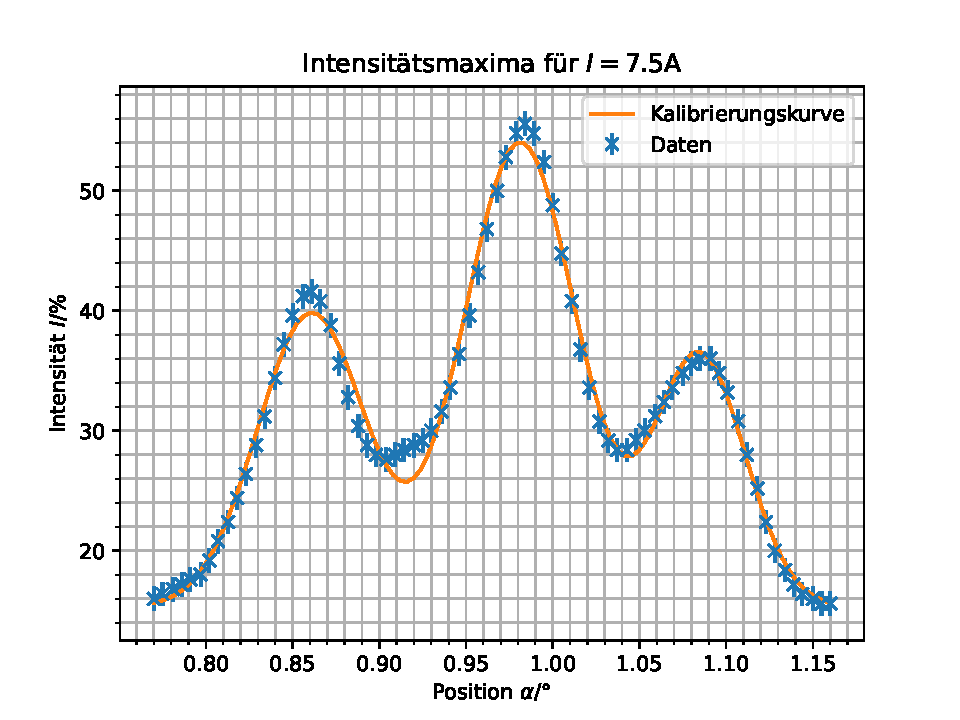
\includegraphics[width=\linewidth]{gauss_7.5A.pdf}
  \end{minipage}
  \hfill
  \begin{minipage}{.49\linewidth}
    \centering
    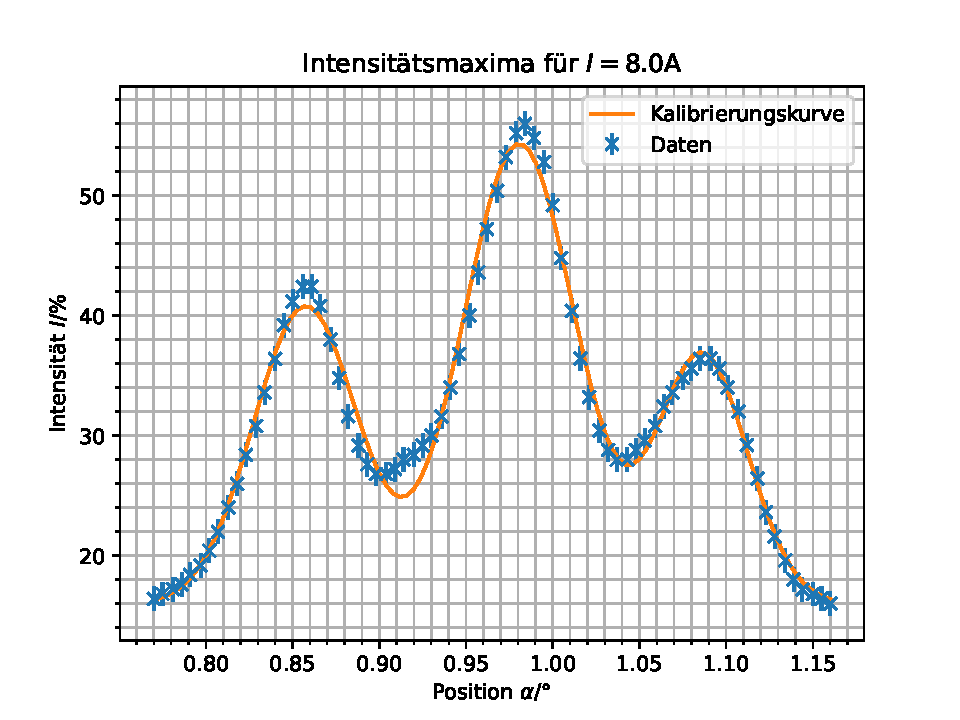
\includegraphics[width=\linewidth]{gauss_8.0A.pdf}
  \end{minipage}

  \begin{minipage}{.49\linewidth}
    \centering
    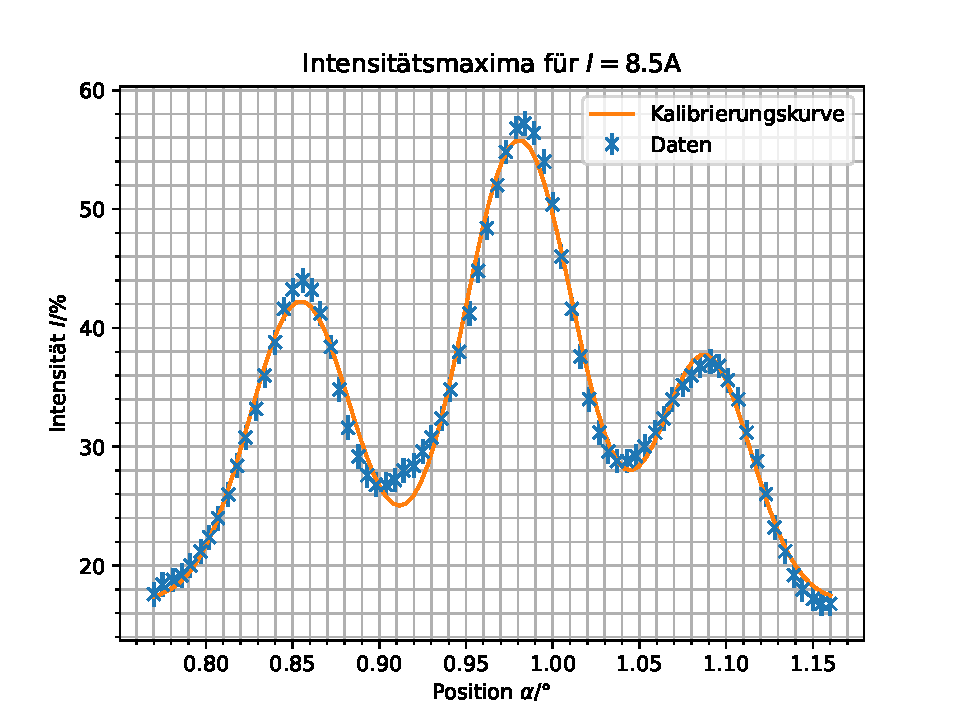
\includegraphics[width=\linewidth]{gauss_8.5A.pdf}
  \end{minipage}
  \hfill
  \begin{minipage}{.49\linewidth}
    \centering
    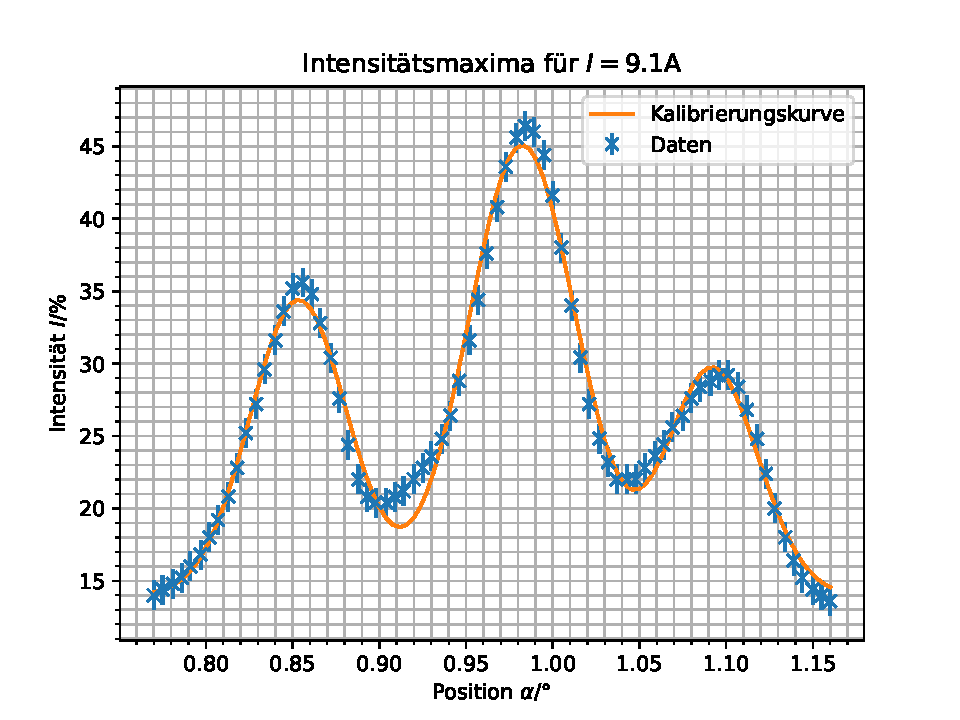
\includegraphics[width=\linewidth]{gauss_9.1A.pdf}
  \end{minipage}
  \caption{Ausgewählte Intensitätsmaxima für verschiedene Magnetströme $I$, mit Gauß-Fit [Teil 2]}
  \label{fig:gauss-fit-2}
\end{figure}

\begin{table}[h]
    % table head=\hline $I$ & $a_1[\%]$ & $\Delta a_1[\%]$ \\ \hline,
    % table head=\hline $I$ & $a_1$ & $\Delta a_1$ & $$ \\,
  \centering
  \csvreader[
    table head=\hline $I$ & $a_1$ & $\Delta a_1$ & $b_1$ & $\Delta b_1$ & $c_1$ & $\Delta c_1$
      $a_2$ & $\Delta a_2$ & $b_2$ & $\Delta b_2$ & $c_2$ & $\Delta c_2$
      $a_3$ & $\Delta a_3$ & $b_3$ & $\Delta b_3$ & $c_3$ & $\Delta c_3$ & $B$ & $\Delta B$\\,
    tabular=|c||c|c|c|c|c|c||c|c|c|c|c|c||c|c|c|c|c|c||,
    late after line=\\\hline,
    head to column names
  ]{../data/zeeman_params.csv}{}%
  {    \csvcoli & \csvcolii & \csvcoliii & \csvcoliv & \csvcolv & \csvcolvi & 
    \csvcolvii & \csvcolviii & \csvcolix & \csvcolx &
    \csvcolxi & \csvcolxii & \csvcolxiii & \csvcolxiv & \csvcolxv &\csvcolxvi & \csvcolxvii & \csvcolxviii & \csvcolxix}

    % \csvcolxvi & \csvcolxvii & \csvcolxviii & \csvcolxix & \csvcolxx}
  % {\csvcoli &\csvcolii &\csvcoliii &\csvcoliv &\csvcolv &\csvcolvi &\csvcolvii &\csvcolviii &\csvcolix &\csvcolx &\csvcolxi}
  %  &\csvcolxii &\csvcolxiii &\csvcolxiv &\csvcolxv &\csvcolxvi &\csvcolxvii &\csvcolxviii &\csvcolxix &\csvcolxx & \csvcolxxi}
  \caption{Bestimmte Parameter der Intensitätsmaxima für verschiedene Ströme}
\end{table}




\begin{thebibliography}{9}

\bibitem{Anleitung}
\textit{Physikalisches Praktikum Teil IV -- Versuchsbeschreibungen}, Universität Bonn, Abruf 29.10.2024

\bibitem{Leybold}
\textit{Beobachtung des normalen Zeeman-Effekts in transversaler und longitudinaler Konfiguration}, Leybold Didactic, Abruf 30.10.2024

\end{thebibliography}


\end{document}

